\documentclass{article1}

\def\vol{00}
\def\issue{000}
\def\copyrightyear{2050}

\usepackage{newtxtext,newtxmath}
%\usepackage{newpxtext,newpxmath}
\usepackage{natbib}
\usepackage[justification=justified]{caption}
\usepackage{booktabs}
\usepackage{placeins}
\usepackage{xcolor}
%\usepackage{pdflscape}
\usepackage{rotating}
\usepackage{xr}
%\externaldocument{bppGDI-SI}

%\bibpunct{[}{]}{,}{n}{}{;}

%\usepackage[switch, modulo]{lineno}
%\linenumbers

\allowdisplaybreaks[2]

\DeclareMathOperator{\E}{\mathbb{E}}
\DeclareMathOperator{\V}{\mathbb{V}}
\newcommand{\U}{\mathbb{U}}
\renewcommand{\P}{\mathbb{P}}
\renewcommand{\d}{\mathrm{d}}
\DeclareMathOperator{\e}{\mathrm{e}}

\newcommand{\red}[1]{{\color{red}{#1}}}
\newcommand{\blue}[1]{{\color{blue}{#1}}}
\newcommand{\pink}[1]{{\color{magenta}{#1}}}
\newcommand{\purple}[1]{{\color{purple}{#1}}}

\begin{document}

\title[Heuristic species delimitation] {A pipeline for heuristic species delimitation
   under the multispecies coalescent model using multilocus sequence data}

\author[Kornai \textit{et~al.}]%
{Daniel Kornai (orcid: 0000-0003-4919-2384)\,$^{1}$, Tom\'{a}\v{s} Flouri (orcid:
0000-0002-8474-9507)\,$^{1}$, and Ziheng Yang (orcid:
0000-0003-3351-7981)\,$^{1,}$\footnote{to whom correspondence should be addressed}}

\address{
	$^1$Department of Genetics, Evolution and Environment, University College London, UK
}

\date{Received on xxxx, revised on xxxx, accepted on xxxx}


\begin{abstract}
The multispecies coalescent (MSC) model accommodates genealogical fluctuations across the
genome and provides a natural framework for comparative analysis of genomic sequence data
to infer the history of species divergence and gene flow.  Given a set of populations,
hypotheses of species delimitation (and species phylogeny) may be formulated as instances
of MSC models (e.g., MSC for one species versus MSC for two species) and compared using
Bayesian model selection. This approach, implemented in the Bayesian program \textsc{bpp},
has been found to be prone to over-splitting. Alternatively heuristic criteria based on
population parameters under the MSC model (such as population/species divergence times,
population sizes, and migration rates) estimated from genomic sequence data may be used to
delimit species.  Here we extend the approaches of \cite{Jackson2017} and
\cite{Leache2019} based on the genealogical divergence index ($gdi$) and develop
hierarchical merge and split algorithms for heuristic species delimitation, and implement
them as a python pipeline.  Applied to data simulated under a model of isolation by
distance, the approach was able to recover the correct species delimitation, whereas model
comparison by \textsc{bpp} failed.  Analyses of empirical datasets suggest that the
procedure may be less prone to the problem of over-splitting.  We discuss possible
strategies for accommodating gene flow in the procedure, as well as the challenges of
species delimitation based on heuristic criteria. \\ %
\textsc{bpp} $|$ genealogical divergence index $|$ multispecies coalescent $|$ species
delimitation
\end{abstract}

\maketitle


\section{Introduction}

Delineation of species boundaries is important to characterizing patterns of biological
diversity, especially during the current global changes in climate and environment.
Traditionally, species have been identified and distinguished using morphological
characteristics.  Molecular genetic data are informative about many processes related to
species delimitation and identification, including population identities, interspecific
hybridization and gene flow, and phylogenetic relationships and and divergence times among
the populations \citep{Fujita2012, Degnan2018, Kubatko2019, Jiao2021MSC}.  Early methods
that use genetic data to identify and delimit species rely on simple genetic-distance
cutoffs (such as the 3x, 4x, or 10x rules), requiring interspecific divergence to be a few
times larger than intraspecific diversit \citep{Hebert2004}, or reciprocal monophyly in
gene trees  \citep[e.g,][]{Sites2004}.  However, such criteria are too simplistic as they
do not accommodate polymorphism in the ancestral populations and incomplete lineage
sorting \citep{Hudson2003} or uncertainties in gene-tree reconstruction
\citep{Knowles2007, Yang2017}.

The multispecies coalescent model \citep{Rannala2003} provides the natural framework for
analysis of sequence data from closely related species or populations.  Likelihood-based
implementations of the MSC accommodate incomplete lineage sorting and stochastic variation
in gene trees (so that reciprocal monophyly is not needed) and gene-tree reconstruction
errors, allowing species delimitation to proceed despite widespread incomplete lineage
sorting or very little phylogenetic information at every locus.

Given a set of populations, different species delimitations correspond to different ways
of merging populations into the same species.  Each species delimitation, combined with
the phylogeny for the delimited species, can be formulated as an instance of the
multispecies coalescent (MSC) model and fitted to genomic sequence data sampled from the
extant species or populations.  Competing models of delimitation can then be compared via
Bayesian model selection (i.e., using posterior model probabilities or Bayes factors) to
find the best supported delimitation \citep{Yang2010}.  In the Bayesian program
\textsc{bpp}, this is accomplished by using a Markov chain Monte Carlo (MCMC) algorithm to
calculate the posterior probabilities for different MSC models \citep{Yang2010, Yang2014,
Yang2015, Flouri2018}. In simulations, \textsc{bpp} showed lower rates of species
overestimation and underestimation than the generalized mixed Yule-coalescent or Poisson
tree processes \citep{Luo2018}.  In empirical datasets, \textsc{bpp} was effective in
identifying cryptic species among ancient lineages.  For example, \cite{Ramirez-Reyes2020}
identified 13 new species of leaf-toed geckoes in a lineage that diverged 30 Ma.

However, the approach of model selection implemented in \textsc{bpp} has often been
noted to over-split, identifying more lineages as distinct species than many other
methods \citep{Sukumaran2017}.  For example, \cite{Campillo2020} analyzed 99 population
pairs in the genus \textit{Drosophila} and found that \textsc{bpp} identified 80 pairs
as distinct species, whereas reproductive isolation was identified in only 69 pairs.
Similarly, \citet{Bamberger2022} examined 48 \textit{Albinaria cretensis} land snail
populations, and found that morphological classifications suggested 3--9 species,
\textsc{admixture} suggested at least 15, while \textsc{bpp} suggested 45--48.
\citet{Barley2018} simulated multiple populations from a single species that exhibits
isolation by distance, and found that \textsc{bpp} delimits geographically separated
populations as distinct species. Those results suggest that the lineages identified by
\textsc{bpp} sometimes correspond to populations rather than species
\citep{Chambers2020}. Multiple studies using \textsc{bpp} have suggested significant
taxonomic reassignments not supported using other methods (e.g., in Yunnan Bananas;
\citealp{Wu2018}).  A number of authors have expressed concerns about the apparent
over-splitting of \textsc{bpp} \citep{MacGuigan2021}.

Rather than treating species delimitation as a model-selection problem, an alternative
approach is to define species status using empirical criteria based on parameters that
characterize the history of population divergence and gene flow, such as the population
split time ($\tau$), population sizes ($\theta_A, \theta_B$), and migration rates
($M_{AB}, M_{BA}$).  Those parameters can be estimated under the MSC from the genomic
data, with the stochasticity of the coalescent process and the phylogenetic uncertainty in
genealogical trees accommodated.  \citet{Jackson2017} introduced a criterion called the
\textit{genealogical divergence index} ($gdi$), by considering the probability that
two sequences sampled from $A$ ($a_1$ and $a_2$) coalesce before either coalesces with a
sequence ($b$) sampled from $B$ (see fig.~\ref{fig:gdi-trees}).  When $a_1$ and $a_2$
coalesce first, the resulting gene tree has the topology $G_1 = ((a_1, a_2), b)$.  Let its
probability be $P_1 = \P(G_1)$.  In the case of no gene flow between $A$ and $B$, this is
given as
\begin{equation} \label{eq:PG1_M0}
   P_1 = \P(G_1|\Theta) = 1 - \tfrac{2}{3} \e^{-2 \tau_{AB} / \theta_A},
\end{equation} 
where the parameter vector is $\Theta = (\tau, \theta_A, \theta_B, \theta_R)$, with
$\tau_{AB} = T_{AB}\mu$ to be the the population divergence time and $\theta_A =
4N_A\mu$ to be the population size of $A$, with $T_{AB}$ to be population split time in
generations, and $\mu$ the mutation rate per site per generation.  Both $\tau$ and
$\theta$ are measured in the expected number of mutations per site.  $P_1$ is a simple
function of $2\tau_{AB}/\theta_A = T_{AB}/(2N_A)$, the internal branch length in the
population phylogeny in coalescent units (with one coalescent time unit to be $2N_A$
generations in population $A$).

$P_1$ of eq.~\ref{eq:PG1_M0} ranges from $\frac{1}{3}$ (when populations $A$ and $B$ are
at panmixia) to 1 (when $A$ and $B$ are completely isolated).  This is rescaled so that
the $gdi$ ranges from 0 to 1 \citet{Jackson2017}:
\begin{equation} \label{eq:gdi}
   gdi = \frac{P_1 - \frac{1}{3}}{1-\frac{1}{3}} = 1 - \e^{-2\tau_{AB} / \theta_A} = 1 - \e^{-T_{AB} / (2N_A)}.
\end{equation} 
A $gdi$ close to 1 indicates a high level of population divergence.  Based on a
meta-analysis of data from \citet{Pinho2010}, \citet{Jackson2017} suggest that
populations are likely to be a single species if $gdi < 0.2$, and separate species if
$gdi > 0.7$.  Intermediate values ($0.2 < gdi < 0.7$) indicate ambiguous species status.

\citet{Leache2019} described a hierarchical merge algorithm for species delimitation based
on $gdi$.  Given a set of populations and a guide tree for them, the procedure
attempts to merge two populations into one species, judged by $gdi$. Here we
develop a python pipeline to automate the procedure.  We include a hierarchical split
algorithm as well.  We first describe the definition and computation of $gdi$ when
there is gene flow in the model, following \citet{Leache2019}.  Then we discuss our new
pipeline and illustrate it using a simulated dataset.  We apply the pipeline to three
empirical datasets, for giraffes, milksnakes, and sunfish.

\begin{figure} [t]
   \centering %
   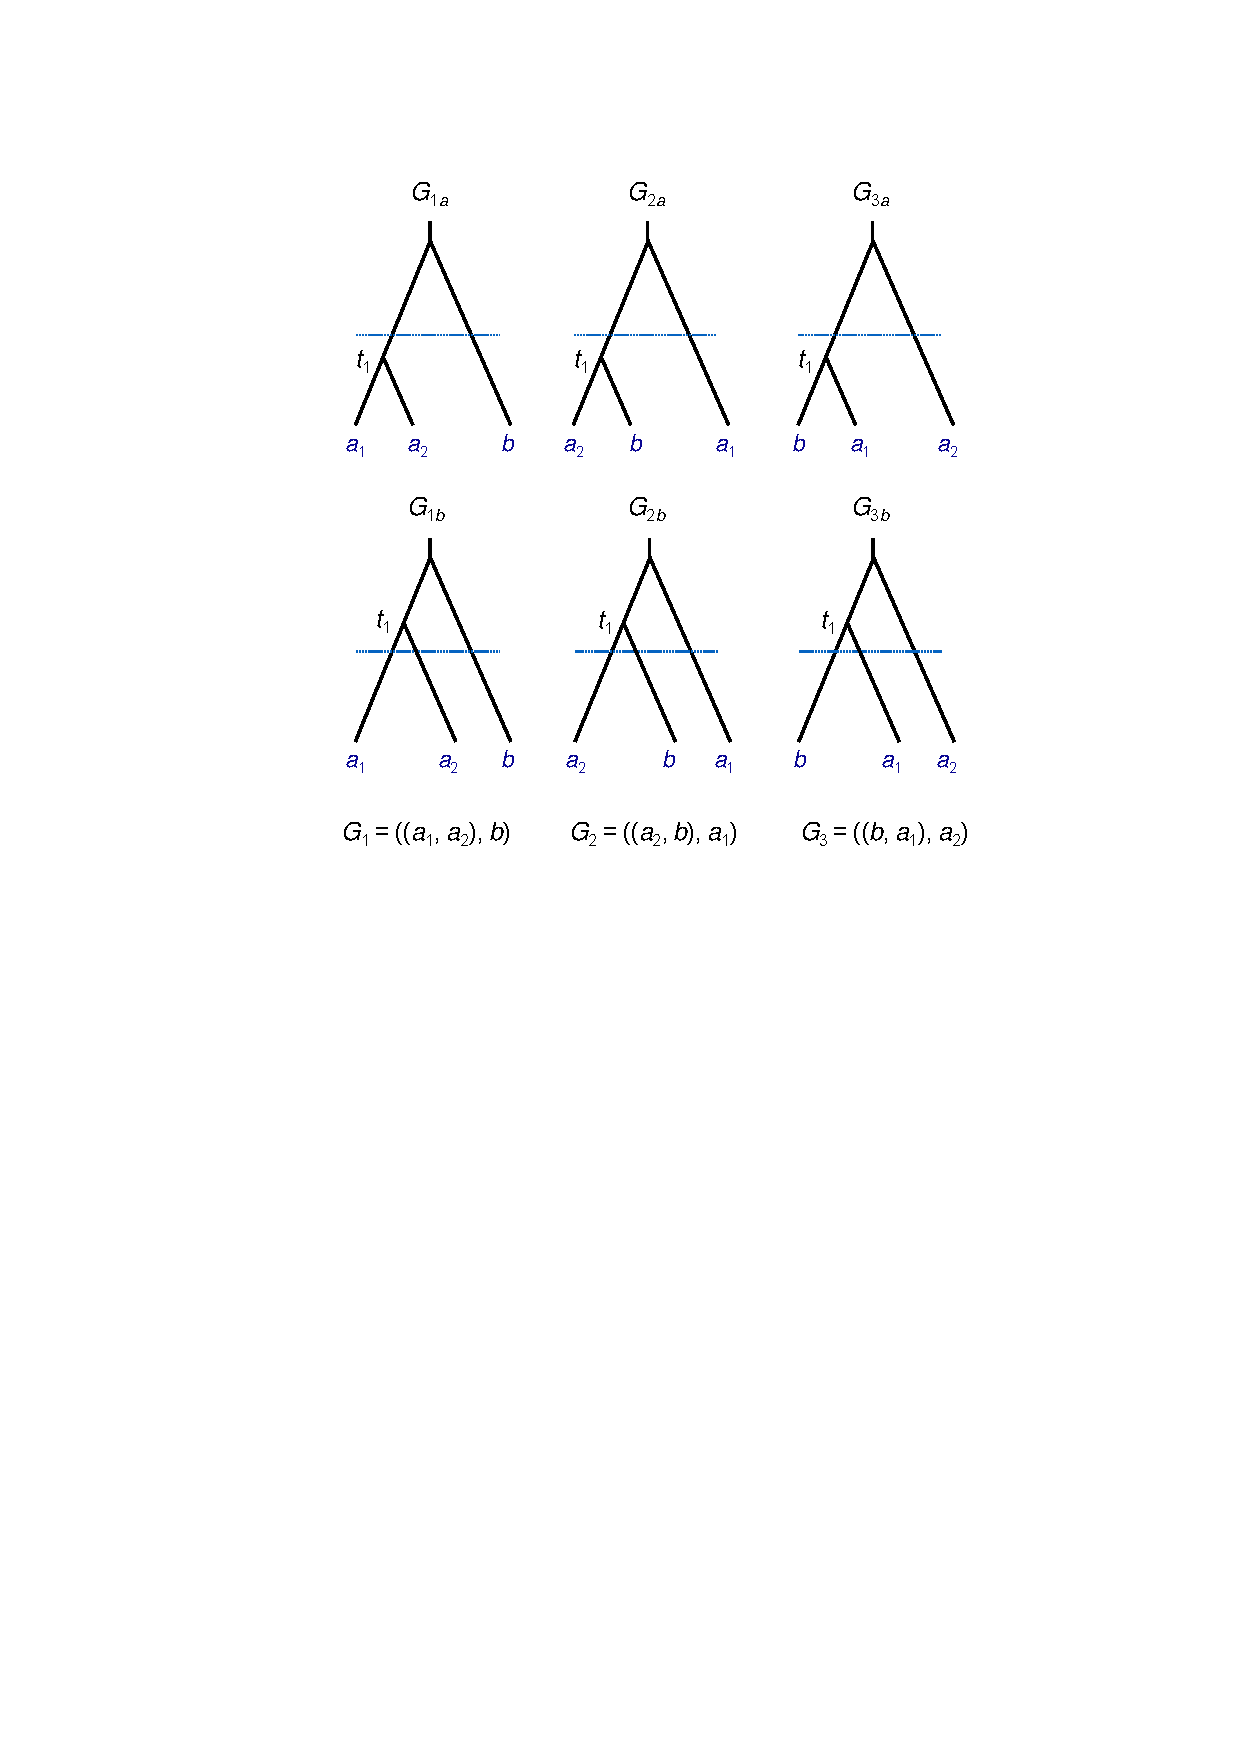
\includegraphics[scale=0.6]{figs/fig-gdi-trees} %
   
   \caption{For a locus with two $A$ sequences and one $B$ sequence ($a_1, a_2, b$), there
   are three possible gene trees: $G_1 = ((a_1, a_2), b)$; $G_2 = ((a_2, b), a_1)$; and
   $G_3 = ((b, a_1), a_2)$.  If the first coalescence is more recent than population
   divergence ($t_1 < \tau$), the gene trees are labelled $G_{1a}, G_{2a}, G_{3a}$;
   otherwise they are labelled $G_{1b}, G_{2b}, G_{3b}$.  The $gdi$ is the
   probability that the two $A$ sequences coalesce first and before the population split:
   $gdi = \P(G_{1a})$.  Note that if there is no gene flow between $A$ and $B$, gene trees
   $G_{2b}$ and $G_{3b}$ are impossible.  %
   } \label{fig:gdi-trees}
\end{figure}


\section{Definition and computation of $gdi$ under the migration model}

\begin{figure} [t]
   \centering %
   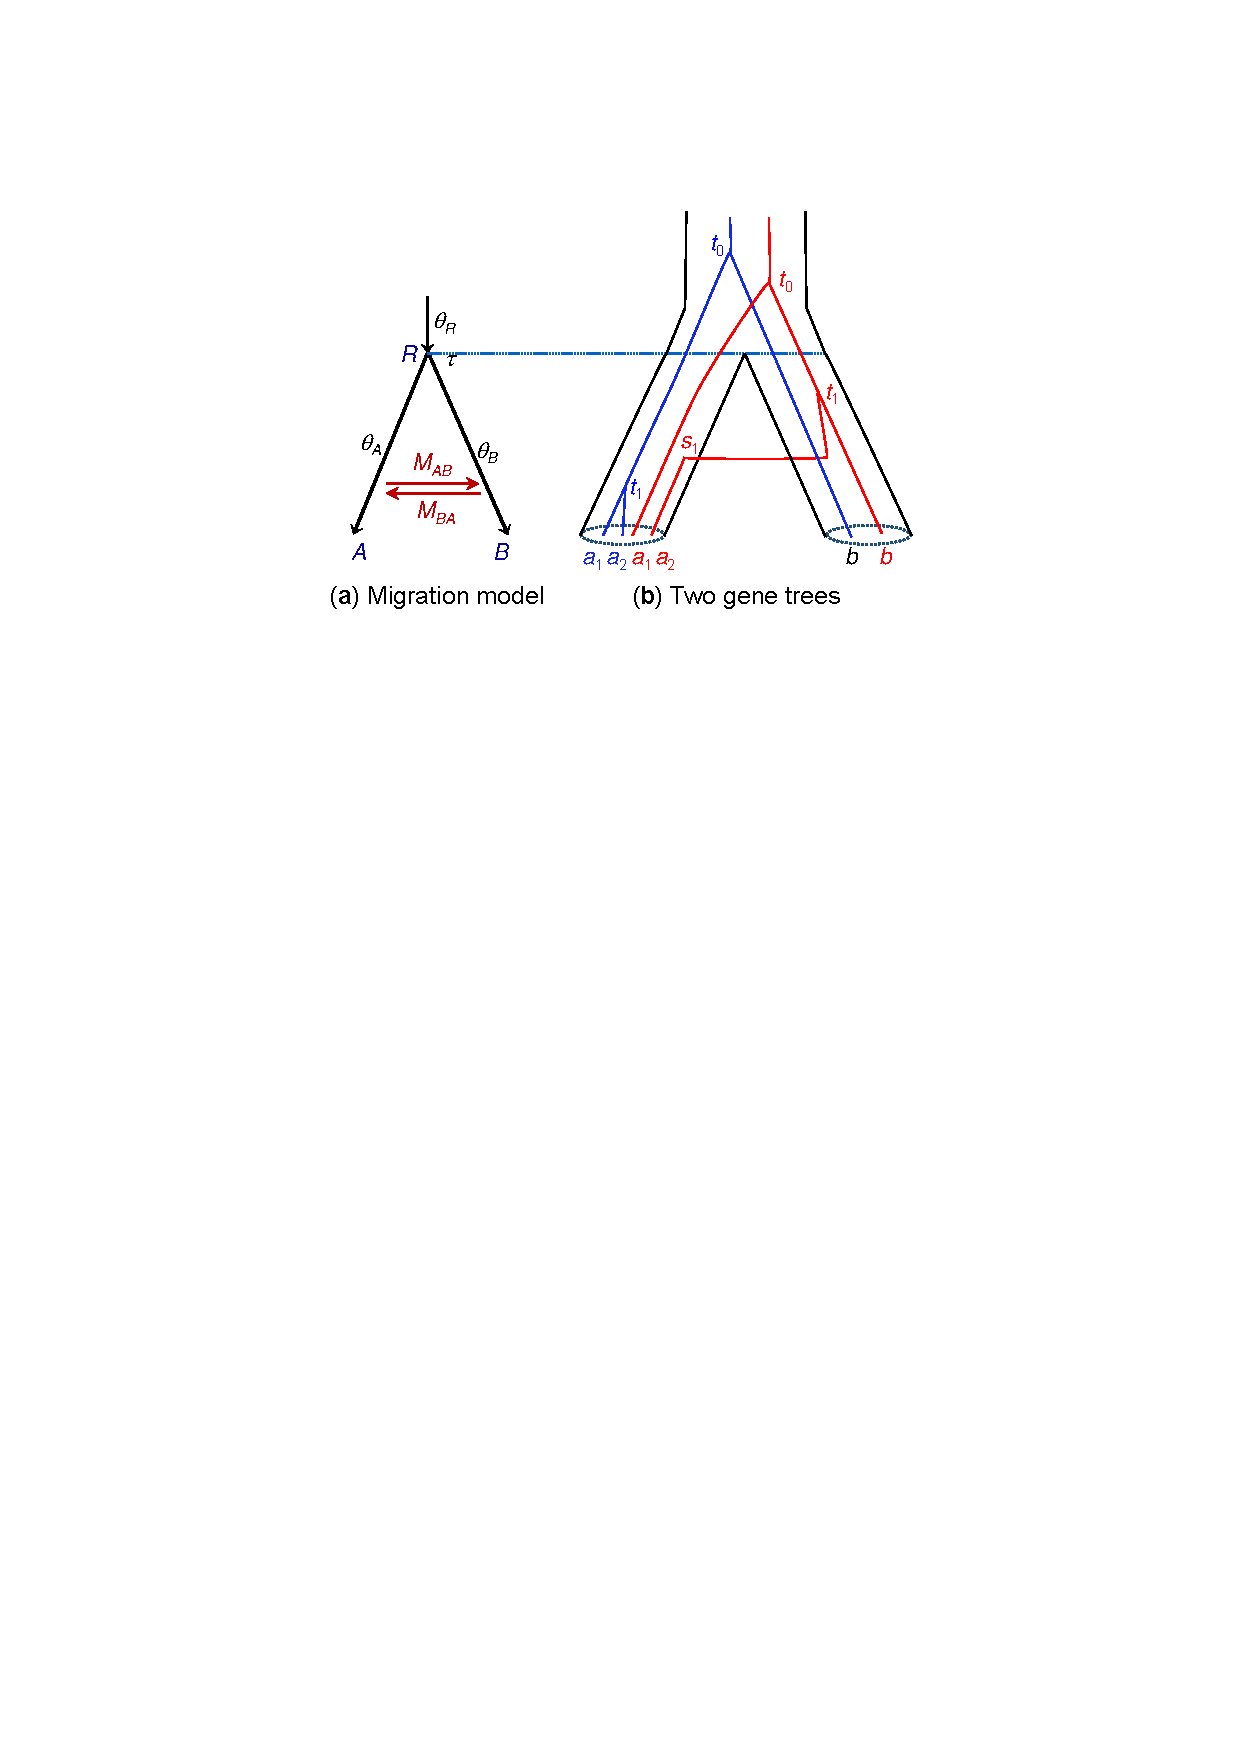
\includegraphics[scale=0.6]{figs/fig-tree-mscm} %
   
   \caption{(\textbf{a}) An MSC-with-migration (MSC-M) model for two species or
   populations ($A,B$) showing the parameters.  The two populations diverged time $\tau
   \equiv \tau_{AB}$ ago and have since been exchanging migrants at the rate of $M_{AB} =
   m_{AB}N_B$ migrants per generation from $A$ to $B$ and at the rate $M_{BA} = m_{BA}N_A$
   from $B$ to $A$.  (\textbf{b}) Two gene trees, each for two $A$ sequences and one $B$
   sequence ($a_1, a_2, b$).  In the blue tree, $a_1$ and $a_2$ coalesce first, in
   population $A$, resulting in the gene tree $G_1 = ((a_1,a_2),b)$ (this is $G_{1a}$ of
   fig.~\ref{fig:gdi-trees}).  In the red tree, $a_2$ migrates into $B$ and coalesce with
   $b$ in $B$, resulting in the gene tree $G_2 = ((a_2,b),a_1)$ (this is $G_{2a}$ of
   fig.~\ref{fig:gdi-trees}). %
} \label{fig:tree-mscm}
\end{figure}

When there is migration between the two populations, the probability for the gene tree
$G_1$ depends on the parameters in the MSC-with-migration (MSC-M) model:
\begin{equation} \label{eq:PG1}
    P_1 = \P(G_1 \bigl| \Theta) ,
\end{equation} 
where $\Theta = (\tau_{AB}, \theta_A, \theta_B, \theta_{AB}, M_{AB}, M_{BA})$ is the
vector of parameters.  \citet{Jackson2017} estimated the minimum and maximum values for
$P_1$ to rescale $P_1$ so that $gdi$ falls into ($0,1$).  Those limits depend on the
model parameters.

Here we instead redefine $gdi$ as the probability that the first coalescence is
between the two $A$ sequences and that it occurs before reaching population divergence
when we trace the genealogy of the three sequences ($a_1, a_2, b$) backwards in time.  In
other words,
\begin{equation} \label{eq:gdi-mscm}
   gdi = \P(G_{1a} \bigl| \Theta) 
\end{equation}
(fig.~\ref{fig:gdi-trees}).  This definition applies whether or not there is gene flow in
the model (fig.~\ref{fig:gdi-trees}), with $0 \le gdi \le 1$; in the case of no gene flow,
eq.~\ref{eq:gdi-mscm} is given by eq.~\ref{eq:gdi}.

Under the MSC-M model, the $gdi$ can be computed analytically, using the Markov
chain characterization of the backward-in-time process of coalescent and migration
\citep{Leache2019}.  For two populations ($A$ and $B$) with gene flow and three sequences
($a_1$, $a_2$, and $b$), the genealogical process of coalescent and migration when one
traces the history of the sample backwards in time can be described by a Markov chain
(table \ref{table:Q}).  The state of the chain is specified by the number of sequences
remaining in the sample and the population IDs ($A$ and $B$) and the sequence IDs ($a_1,
a_2, b$) \citep{Hobolth2011, Zhu2012, Jiao2021}.  For example, The initial state is
$A_{a_1}A_{a_2}B_b$, with three sequences $a_1, a_2, b$ in populations $A$, $A$, and $B$,
respectively.  This is also written `$AAB$'.  State $A_{a_1a_2}B_b$, abbreviated `$AB_b$',
means that two sequences remain in the sample, with the ancestor of $a_1$ and $a_2$ in $A$
and $b$ in $B$.  Finally state $A|B$ is an artificial absorbing state, in which all three
sequences have coalesced with the sole ancestral sequence in either $A$ or $B$.  There are
21 states in the Markov chain, with the transition rate (generator) matrix $Q =
\{q_{ij}\}$ given in table \ref{table:Q}.

The transition probability matrix over time $t$ is then $P(t) = \{p_{ij}(t)\} = \e^{Qt}$,
where $p_{ij}(t)$ is the probability that the Markov chain is in state $j$ at time $t$ (in
the past) given that it is in state $i$ at time 0 (the present time).  Suppose $Q$ has the
spectral decomposition
\begin{equation} 
    q_{ij} = \sum_{k=1}^{21} u_{ik} v_{kj} \lambda_k ,
\end{equation} 
where $0 = \lambda_1 > \lambda_2 \ge \cdots \ge \lambda_{21}$ are the eigenvalues of
$Q$, and columns in $U = \{u_{ij}\}$ are the corresponding right eigenvectors, with $V =
\{v_{ij}\} = U^{-1}$.  Then
\begin{equation} \label{eq:pij}
    p_{ij}(t) = \sum_{k=1}^{21}  u_{ik} v_{kj} \e^{\lambda_k t}.
\end{equation}

Consider the coalescent time $t$ between sequences $a_1$ and $a_2$ given that they are to
coalesce first and before $\tau$ (as in the blue gene tree of figure \ref{fig:tree-mscm}b).
This has density
\begin{equation} \label{eq:ft} 
\begin{aligned}
  f(t) &= \bigl[ p_{AAB, AAA}(t) + p_{AAB, AAB}(t) \bigr] \tfrac{2}{\theta_A} \\
       &+ \bigl[ p_{AAB, BBA}(t) + p_{AAB, BBB}(t) \bigr] \tfrac{2}{\theta_B}, \ \ t < \tau.
\end{aligned}
\end{equation} 
The two terms in the sum correspond to coalescence between $a_1$ and $a_2$ occurring in
populations $A$ and $B$, respectively.  The first term is the probability that $a_1$ and
$a_2$ are in $A$ right before time $t$ (states $AAA$ or $AAB$ depending on whether $b$ is
in $A$ or $B$), times the rate for them to coalesce, $\frac{2}{\theta_A}$. Similarly the
second term is the probability density that $a_1$ and $a_2$ coalesce at time $t$ in $B$.

By averaging over the distribution of $t$, we have 
\begin{equation} \label{eq:gdi-ft} 
    gdi = \int_0^\tau f(t) \; \d t .
\end{equation}
To calculate the integral in eq.~\ref{eq:gdi-ft}, note that from eq.~\ref{eq:pij},
\begin{equation} 
   \begin{aligned}
      \int_0^\tau p_{ij}(t) \,\d t = 
       u_{i1} v_{1j}\tau %
       + \sum_{k=2}^{21} u_{ik} v_{kj} \frac{\e^{\lambda_k \tau} - 1}{\lambda_k} .
   \end{aligned}
\end{equation}

We have implemented this calculation of $gdi$ in the python pipeline for the case
where the two populations are sister lineages exchanging migrants between themselves but
not with other populations.

When populations $A$ and $B$ are involved in gene flow with other populations,
analytical calculation of the $gdi$ becomes complicated.  It is simpler to simulate gene
trees for sequences $a_1, a_2, b$ under the extended migration model involving more than
two populations to calculate the $gdi$.  Specifically, given the fully specified MSC-M
model for all species/populations (including the species tree topology and parameters
such as $\tau$, $\theta$, $M$), simulate the gene trees with branch lengths (coalescent
times) for a large number of loci ($R = 10^6$, say) , at which three sequences ($a_1,
a_2, b$ ) are sampled.  The $gdi$ is simply the proportion of loci at which the gene
tree is $G_{1a}$, that is, $G_1$ with $t_1 < \tau_{AB}$
(figs.~\ref{fig:gdi-trees}\&\ref{fig:tree-mscm}).


\section{The hierarchical merge and split algorithms}

\begin{figure}[t]
   \centering %
   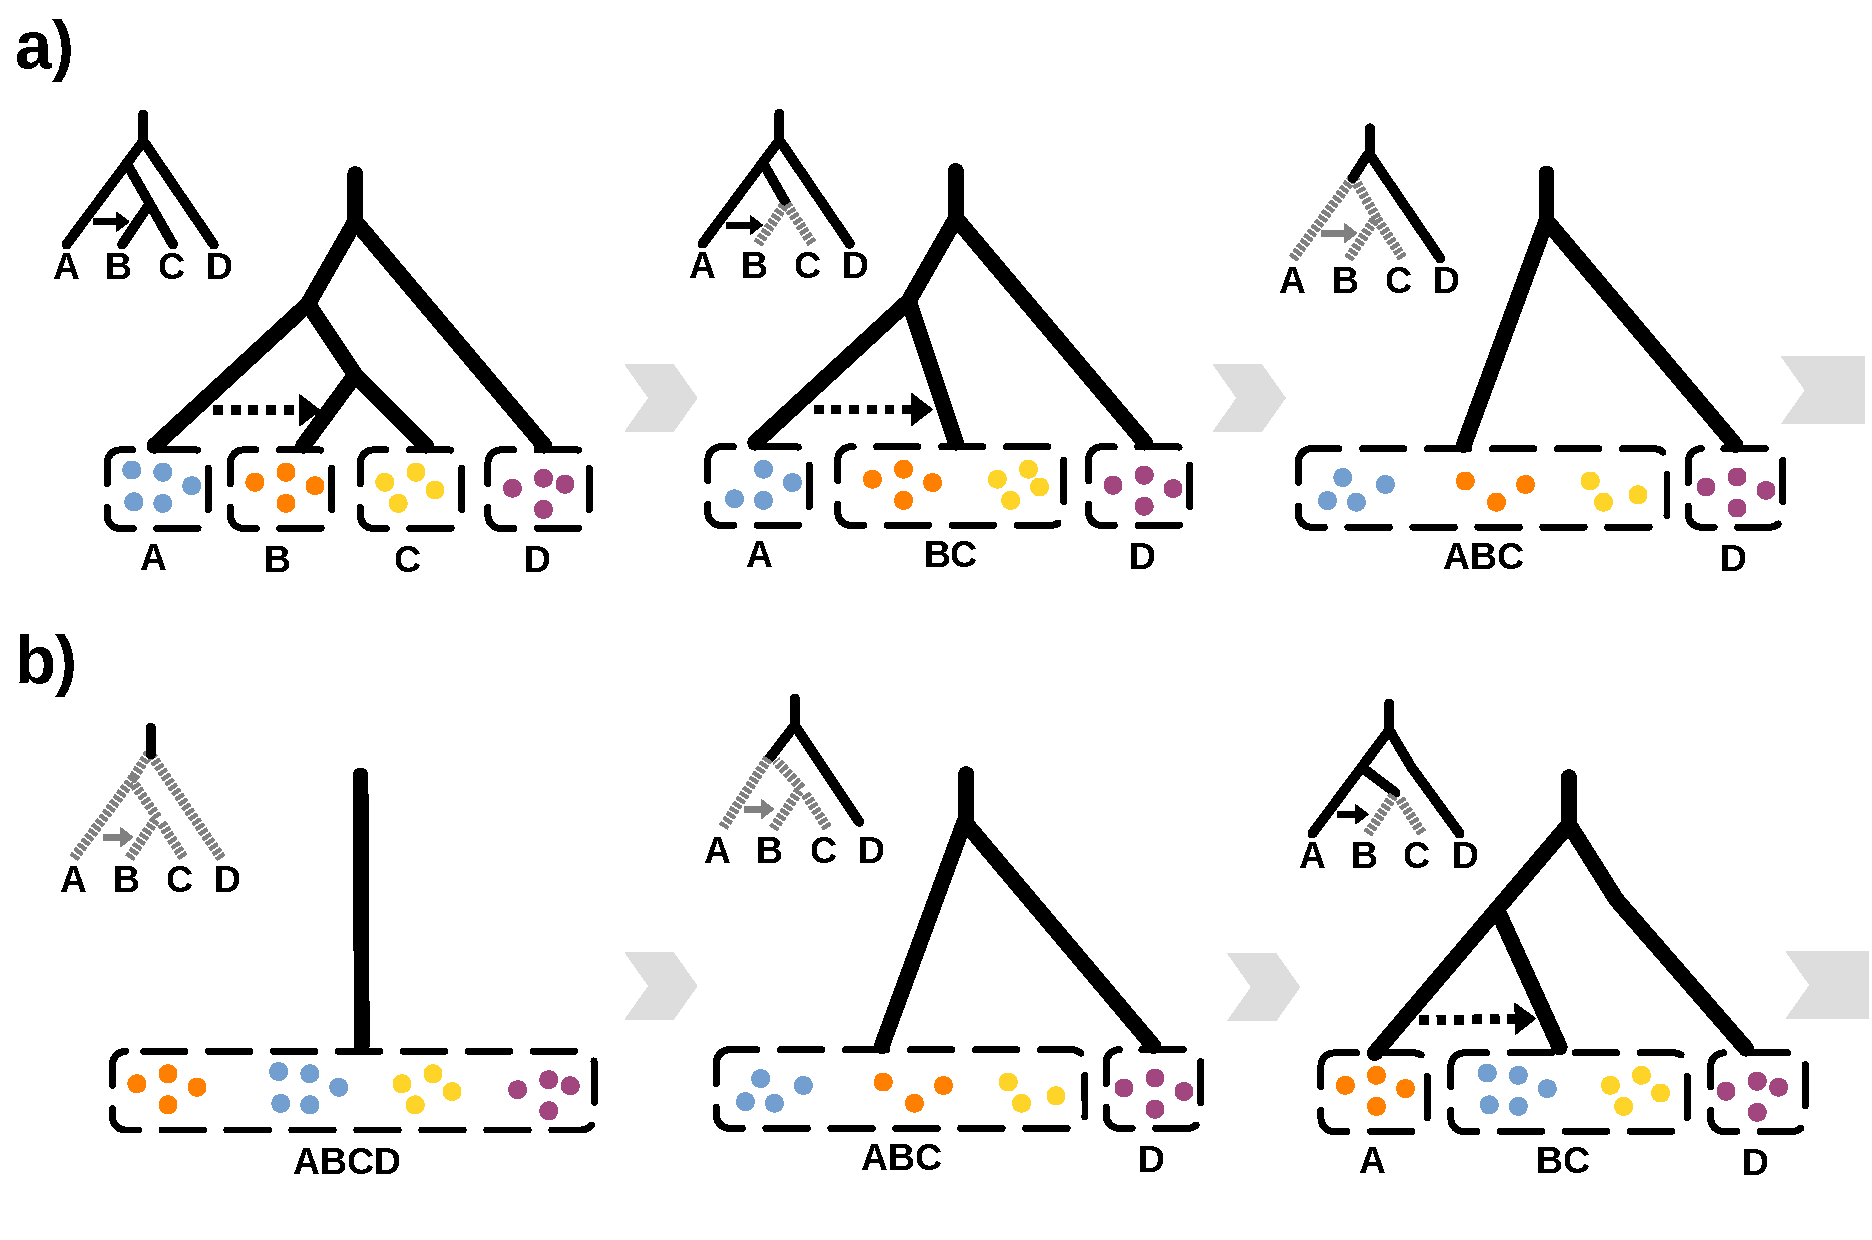
\includegraphics[scale=0.25]{figs/Methods/HM_algo} %
   
   \caption{(\textbf{a}) Hierarchical merge and (\textbf{b}) hierarchical split
   algorithms applied to the same guide tree for four populations. \\%
	} 
	\label{fig:gdi-algorithms}
\end{figure}

We implement both the hierarchical merge and hierarchical split algorithms in a python
pipeline (fig.~\ref{fig:gdi-algorithms}).  Both algorithms require a guide tree for
populations, possibly with migration events.  In the merge algorithm, we progressively
merge the populations into the same species, starting from the tips of the tree and moving
towards the root.  The merge is accepted if and only if the $gdi < 0.2$ for the
population pair.  The algorithm stops when no population pair can be merged
(fig.~\ref{fig:gdi-algorithms}a).

In the hierarchical split algorithm, we start from the MSC model of one species and
progressively split each species into distinct species, starting from the root and moving
towards the tips of the tree (fig.~\ref{fig:gdi-algorithms}b).  The split is accepted if
and only if the $gdi > 0.7$.  The algorithm stops when no species can be split
(fig.~\ref{fig:gdi-algorithms}b).

Both algorithms are implemented under either the MSC model with no gne flow or the MSC-M
model with continuous migration.  Under the MSC-M model, we retain the migration event
when populations are merged as long as there is migration between the subpopulations.  For
example, there is migration from $A$ to $B$ in the guide tree (the initial delimitation)
(fig.~\ref{fig:gdi-algorithms}a).  Later when $B$ and $C$ are merged into one
species/population, we retain the migration event (now from population $A$ to population
$BC$).


\section{Example with simulated data ($ABCDX$)}

\begin{figure}[t]
   \centering
   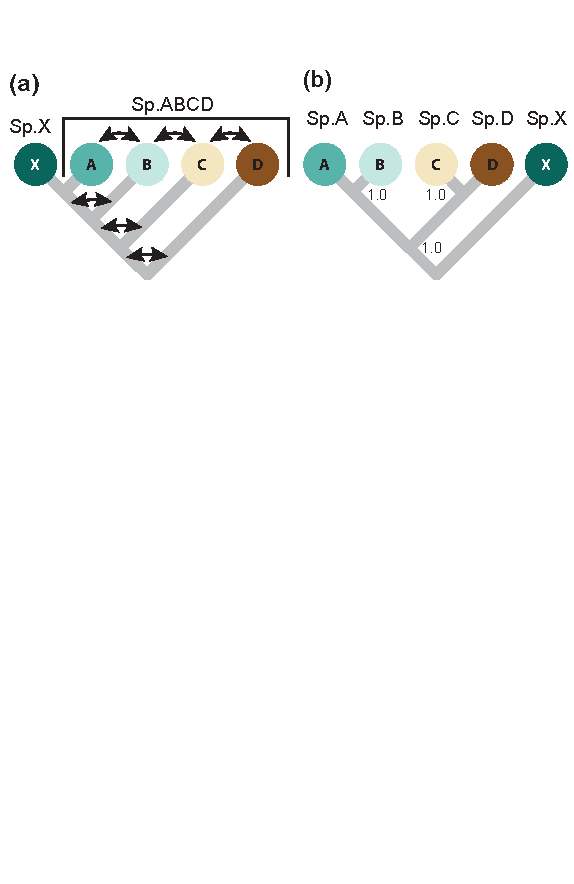
\includegraphics[scale=0.7]{figs/fig-ABCDX}
   
   \caption{(\textbf{a}) An isolation-by-distance model used to simulate multilocus
   sequence data, in which $A, B, C, D$ represent populations of a widely distributed
   species while $X$ is a new species that split off from population $A$.  (\textbf{b})
   Incorrect species delimitation and phylogeny in Bayesian model selection using
   \textsc{bpp} under the MSC model assuming no gene flow.  Use of the guide tree and the
   $gdi$ criterion leads to delimitation of two species.  Redrawn after
   \citet[][fig.~5]{Leache2019}. %
} \label{fig:ABCDX}
\end{figure}

\citet{Leache2019} simulated sequence data under the MSC-with-migration model for five
populations of figure \ref{fig:ABCDX}, in which $A, B, C, D$ represent geographical
populations for a paraphyletic species distributed across a wide geographic range while
$X$ is a new species that split off from population $A$. Migration between any two
neighbouring populations of species $ABCD$ occurs at the rate of $M = Nm = 2$ migrants
per generation, whereas there is no gene flow involving $X$.  The data consisted of
$L=100$ simulated loci, with two sequences sampled per species per locus, and 500 sites
in the sequence.  We use the dataset to illustrate our pipeline, and to discuss the
challenges of species delimitation in presence of gene flow.

The control file for the program can be found in figure \ref{fig:ABCDX_mcf}.  During the
analysis, the pipeline provides feedbacks about the current species delimitation and the
decisions made during each iteration
(figs.~\ref{fig:ABCDX_out}\&\ref{fig:ABCDX_text_out}).  During the first iteration,
attempt was made to merge the two current leaf node pairs ($A,B$, and $C-D$).  As $gdi
<0.2$ for each pair, the merge was accepted.  In the second iteration, a merge between
the pair $AB$ and $CD$ was attempted, and again this was accepted.  In the third
iteration, a merge between the pair $ABCD$ and $X$ was attempted.  As $gdi > 0.2$, the
merge was rejected.  The final delimitation has two species, $ABCD$ and $X$.

\begin{figure}[t]
	\centering %
	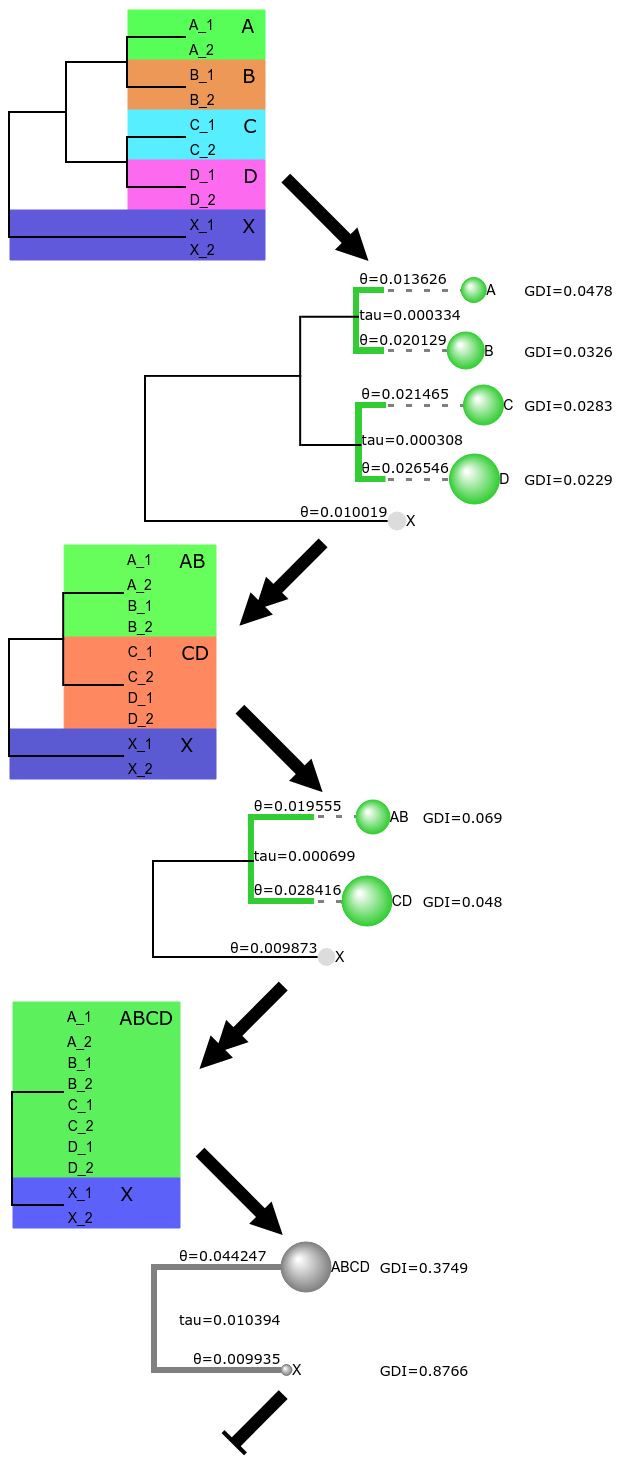
\includegraphics[scale=0.30]{figs/Pipedemo/sim_fig_v1} %
	
   \caption{Screen output produced by the pipeline during the hierarchical merge iteration
   showing the currently accepted species delimitation and species phylogeny with
   parameter estimates ($\tau, \theta$). %
   } \label{fig:ABCDX_out}
\end{figure}


\section{Empirical examples}

\subsection{Species delimitation in the genus Giraffa}

\begin{figure}[t]
    \centering %
    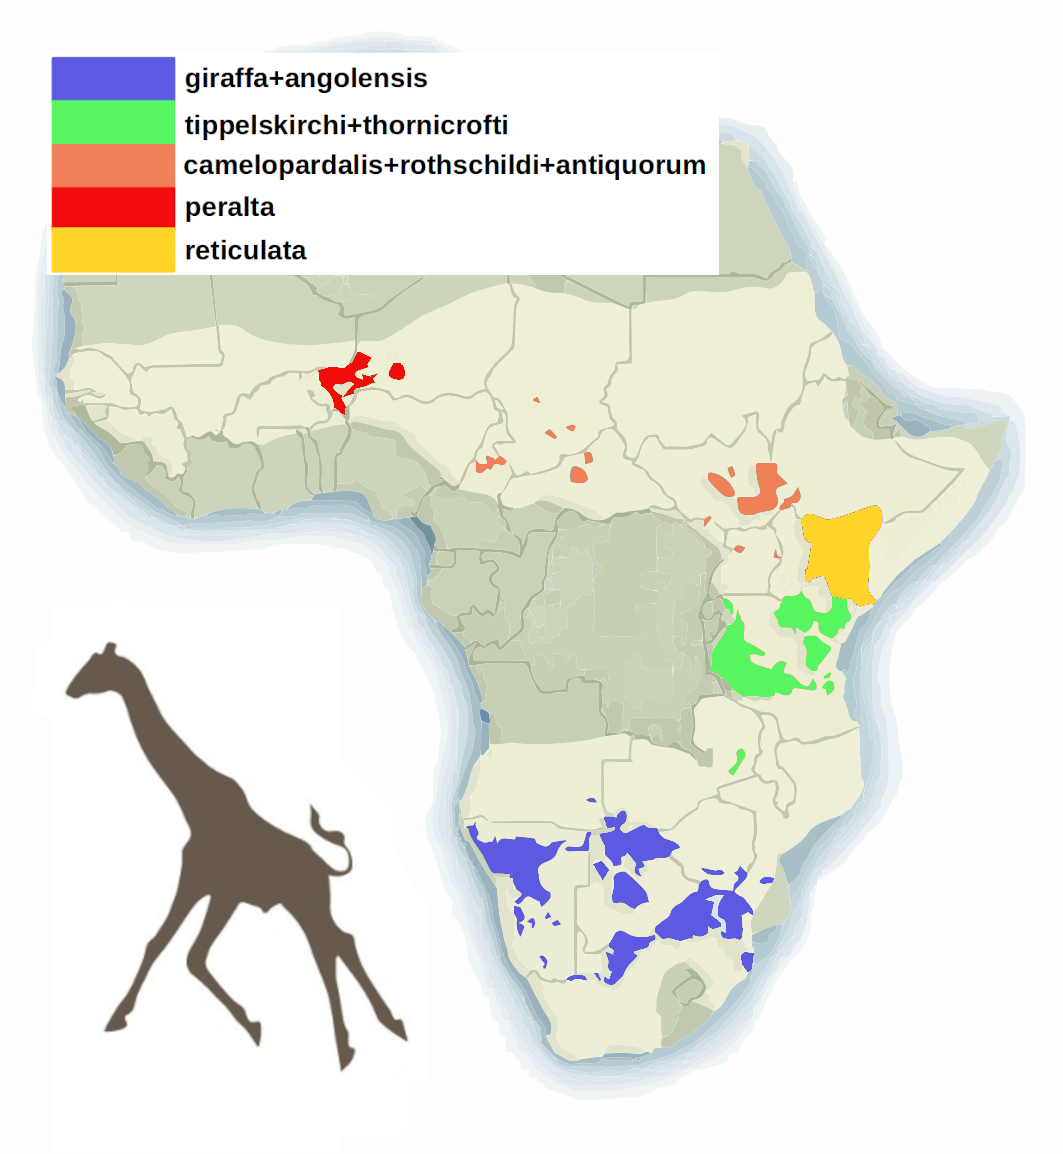
\includegraphics[scale=0.50]{figs/Giraffe/giraffe_fig} %
    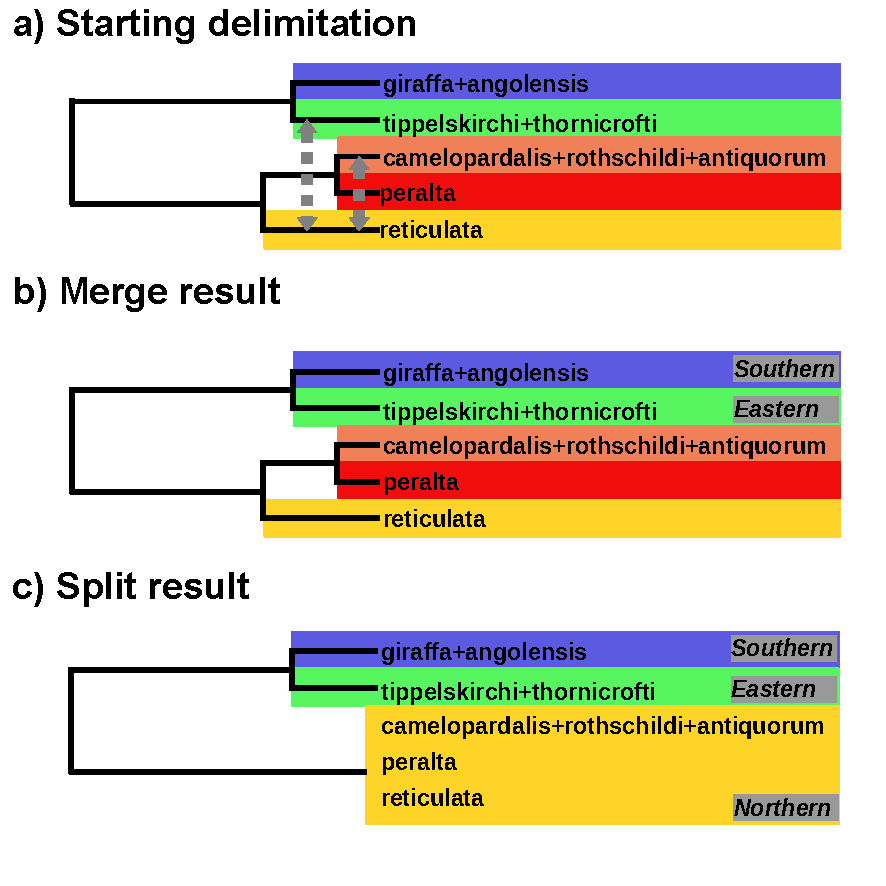
\includegraphics[scale=0.50]{figs/Giraffe/giraffe_result}  %
    
    \caption{Geographical distributions of five species within Giraffa. Bright region on map shows historical (ca. 1700) giraffe ranges (modified from https://giraffeconservation.org/giraffe-species/). %
    (\textbf{a}) The guide tree for five populations of giraffes, with dotted lines
    indicating bidirectional migration events
    \citep[][fig.~1]{Petzold2020}.  %
    (\textbf{b}) The merge algorithm supports five species, while (\textbf{c}) the split
    algorithm supports three. %
    \blue{[Updated figure to use custom image. Updated colours to match between geographic distributions, and the phylogenetic trees.]}
} \label{fig:giraffe}
\end{figure}

Species delimitation in the genetically isolated, but phenotypically convergent Giraffes
has generated considerable controversy \citep{Fiser2018}.  There are nine subspecies
recognised: \textit{camelopardalis}, \textit{angolensis}, \textit{antiquorum},
\textit{giraffa}, \textit{peralta}, \textit{reticulata}, \textit{rothschildi},
\textit{thornicrofti} and \textit{tippelskirchi}, which have been classified into
one to six species in previous studies which used morphological characters and molecular
data. \citet{Petzold2020} compiled a multilocus dataset of 21 introns (average sequence
length 808 bp), sampled from 66 individuals from the nine subspecies, and conducted a
number of population genetic and phylogenetic analyses. \blue{The authors concluded that the best supported number of species is three, and found that \textsc{bpp} supports as many as five species.}

\blue{This five species phylogeny (Fig. \ref{fig:giraffe}a ) is used as the starting delimitation in our analysis.} Based on phylogenetic analysis of mitochondrial haplotypes and hybridized individuals \citep{Fennessy2016, Petzold2020}, bidirectional migration was specified between
\textit{tippelskirchi+thornicrofti} and \textit{reticulata}, and between \textit{reticulata} and \textit{camelopardalis+rothschildi+antiquorum}.  The migration rate was assigned the gamma prior G($1,100$) with mean 0.01 migrant individuals per generation.  Merge and split analyses were conducted with the animal-specific $gdi$ thresholds of 0.3 and 0.7, as recommended by \citet{Jackson2017} (control files in
figs.~\ref{fig:giraffe_mcf_merge} \& \ref{fig:giraffe_mcf_split}).  

\blue{The merge algorithm suggested five species while the split algorithm suggested three
(fig.~\ref{fig:giraffe}). Both methods recognized the Eastern (\textit{thornicrofti} and
\textit{tippelskirchi} and Southern (\textit{angolensis}
and \textit{giraffa}) species present in the starting delimitation as distinct species. For the remaining Northerns populations, the merge algorithm recognized three distinct species (fig.~\ref{fig:giraffe}b),
while the split algorithm recognized only a single Northern species combining the populations (fig.~\ref{fig:giraffe}c).} 

\red{[Also it maybe interesting to look at the estimates of parameters ($\tau, \theta, M$).]}
\blue{The migration rates interred during the delimitation process support the originally hypothesised patterns of hybridization and introgression between reticulated giraffes and their neighbouring populations (fig.~\ref{fig:giraffe_migration}). The highest levels of gene flow occurred within the Northern populations from \textit{cam.+rot.+ant.} to \textit{reticulata}, which notably affected four of the 21 introns in this dataset \citep{Petzold2020}]}

\begin{figure}[h]
	\begin{center}
		\begin{tabular}{|c  c  c |} 
			\hline
			Source & Destination & M \\ 
			\hline
			tip.+tho. & reticulata & 0.0024 \\ 
			reticulata & tip.+tho. & 0.0016 \\
			reticulata & cam.+rot.+ant. & 0.0272 \\
			cam.+rot.+ant. & reticulata & 0.1233 \\
			\hline
		\end{tabular}
	\end{center}
	\caption{Migration rates between the five giraffe species in the starting delimitation. %
	} \label{fig:giraffe_migration}
\end{figure}


\subsection{Species delimitation in milksnakes (\textit{Lampropeltis triangulum})}

\begin{figure}[t]
    \centering %
    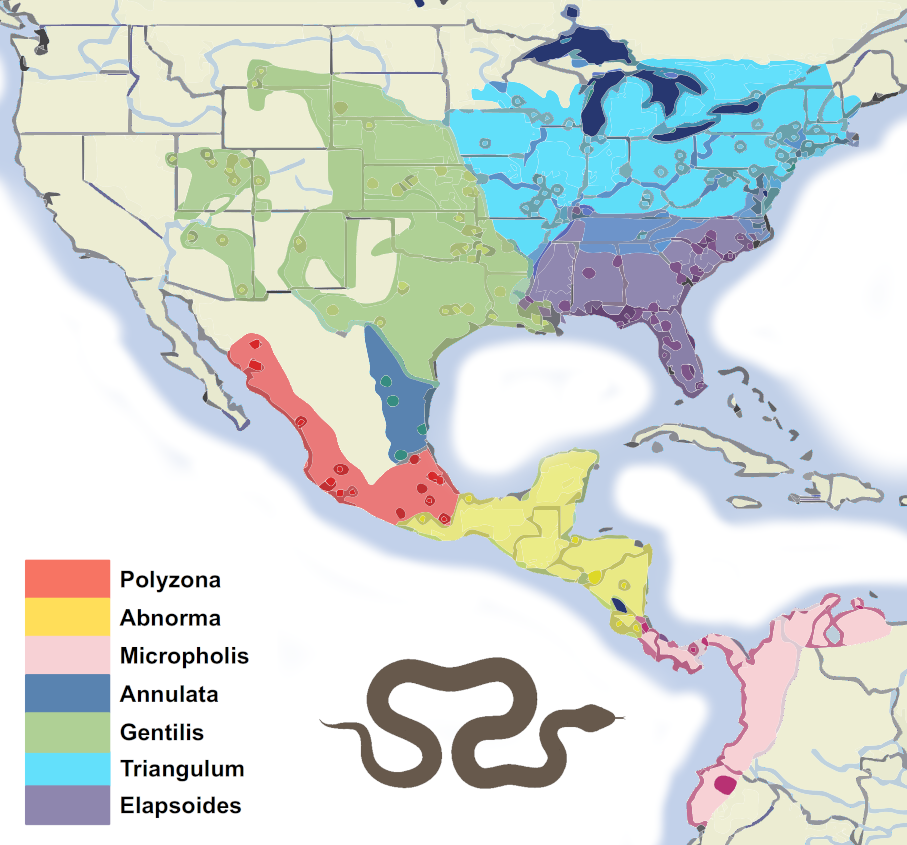
\includegraphics[scale=0.6]{figs/Lampro/figure} %
    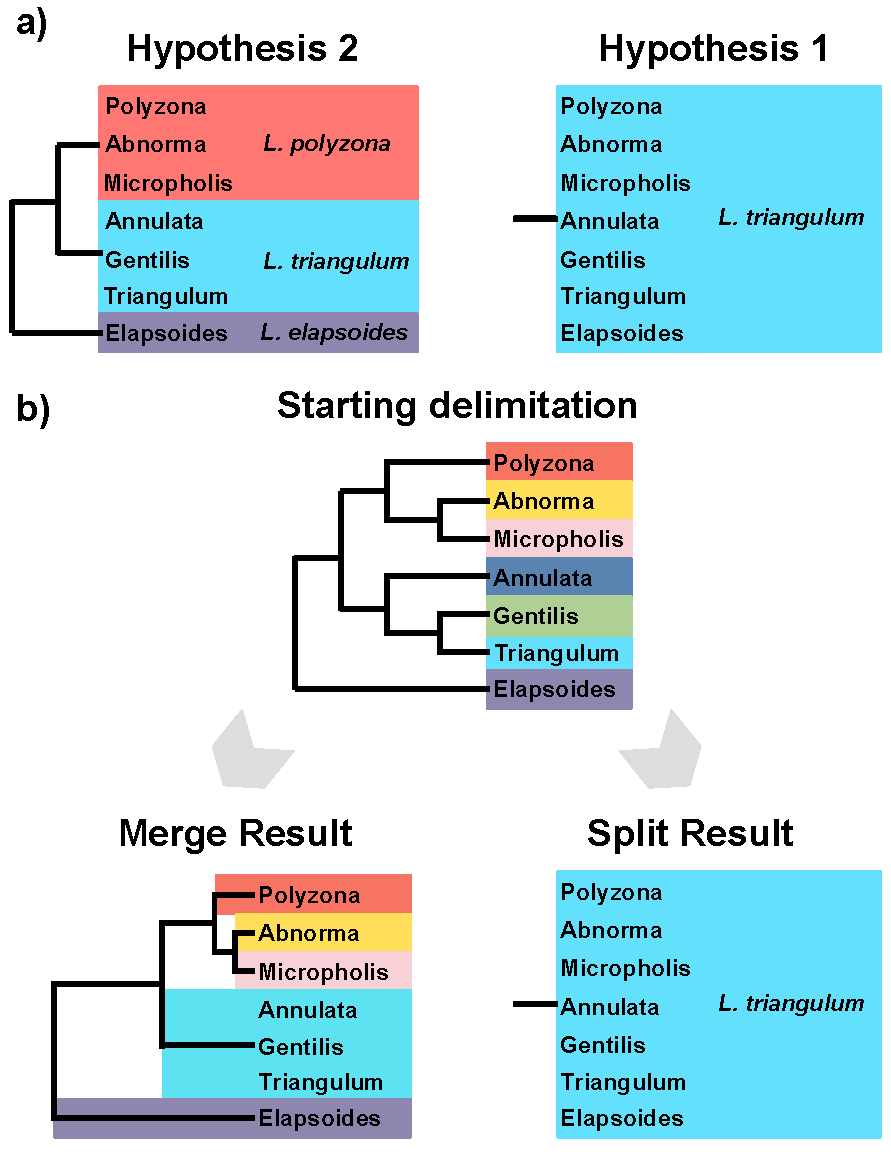
\includegraphics[scale=0.5]{figs/fig-miksnakes-results} %
    
    \caption{\textbf{a)} The one-species and three-species delimitation hypotheses for
    milksnakes suggested by \citet{Chambers2020}.
    \textbf{b)} Starting delimitation, and inferred delimitations using the merge and
    split algorithms. \blue{[Updated figure to use custom image. Updated colours to match between geographic distributions, and the phylogenetic trees.]} %
} \label{fig:milksnake}
\end{figure} 

The American milksnake \textit{Lampropeltis triangulum} is a New World snake with one of
the widest known geographic distributions within the squamates.  Seven subspecies are
known: \textit{abnorma}, \textit{polyzona}, \textit{micropholis}, \textit{triangulum},
\textit{gentilis}, \textit{annulata}, and \textit{elapsoides} (fig.~\ref{fig:milksnake}a).
\citet{Ruane2014} analyzed 11 nuclear loci (average length 537 bp) for 164 individuals
from the seven subspecies using \textsc{bpp} and found evidence for seven distinct
species.  \citet{Chambers2020} suggested that several species hypothesized by
\citet{Ruane2014} may represent arbitrary slices of continuous geographic clines.  Based
on a combination of population genetic and phylogeographic evidence, they suggested two
delimitation hypotheses, with one and three species, respectively
(fig.~\ref{fig:milksnake}\textbf{a}).  \citet{Chambers2020} also constructed five
arbitrary delimitation hypotheses, each with two species representing arbitrary east-west
splits of the \textit{gentilis} and \textit{triangulum} populations.  All the five
delimitation hypotheses were supported by Bayesian model selection using \textsc{bpp}
(fig.~\ref{fig:milksnake_EW}), even though they are not mutually compatible.

We reanalyzed the data using our pipeline, using a guide tree for five populations of
\citet{Chambers2020}, with no migration rates assumed (fig.~\ref{fig:milksnake}).  Merge
and split algorithms were run using $gdi$ thresholds of 0.3 and 0.7 (control files
in \ref{fig:milksnake_mcf_merge} and \ref{fig:milksnake_mcf_split}).  The merge algorithm
established an upper bound of five species.  When compared with the three-species
hypothesis of \citet{Chambers2020}, two of the species (\textit{elapsoides} and
\textit{triangulum}) were identical, but the \textit{polyzona} lineage is split into
distinct species.  The split analysis supported only a single species.

\begin{figure}[t]
	\centering %
	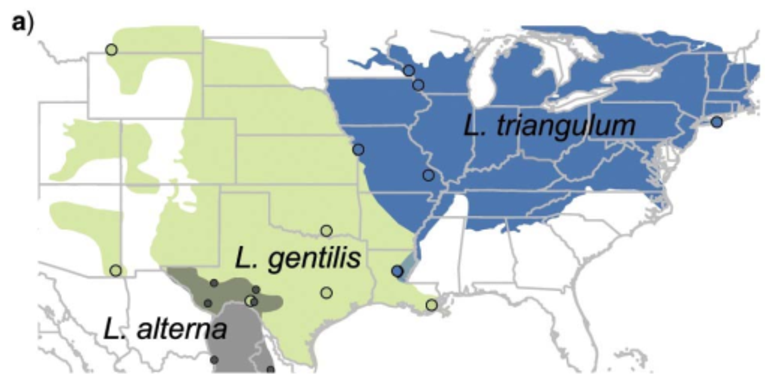
\includegraphics[scale=0.5]{figs/miksnakes_EW} %
	
	\caption{East-West splits for the milksnakes.  Coloured dots represent the sampling
	location and original classification of individuals (blue: \textit{triangulum}, green:
	\textit{gentilis}). %
	} \label{fig:milksnake_EW}
\end{figure} 

We conducted a second analysis using only the 38 individuals from the \textit{gentilis},
\textit{triangulum}, and \textit{alterna} populations (which acted as an outgroup in all
analyses).  The assignment of individuals to the \textit{gentilis} and \textit{triangulum}
populations was varied in each analysis, according to the five arbitrary East-West splits
of \cite{Chambers2020} (fig.~\ref{fig:milksnake}).  Merge and split analyses were ran
using the settings as above (control files available in \ref{fig:milksnake_EW_mcf} and
\ref{fig:milksnake_EW_shell}).

For all five of the East-West splits tested, our merge and split analyses converged on an
identical result, merging the \textit{gentilis} and \textit{triangulum} populations into a
single species.  These results are consistent with the suggestions of \cite{Chambers2020}.

\red{[Comment on the $\sim$0 estimates of migration rates between geographic populations.]}\blue{[As patterns of hybridization or migration for nuclear genes were not specified in the Chambers and Hillis paper, and only nuclear genes were used in the analysis, the model was run without migration (just MSC), thus no migration rates were estimated (See control files in S5 an S6)]}


\subsection{Introgression and species delimitation in the longear sunfish (\emph{Lepomis
megalotis}).}

\begin{figure}[t]
    \centering %
    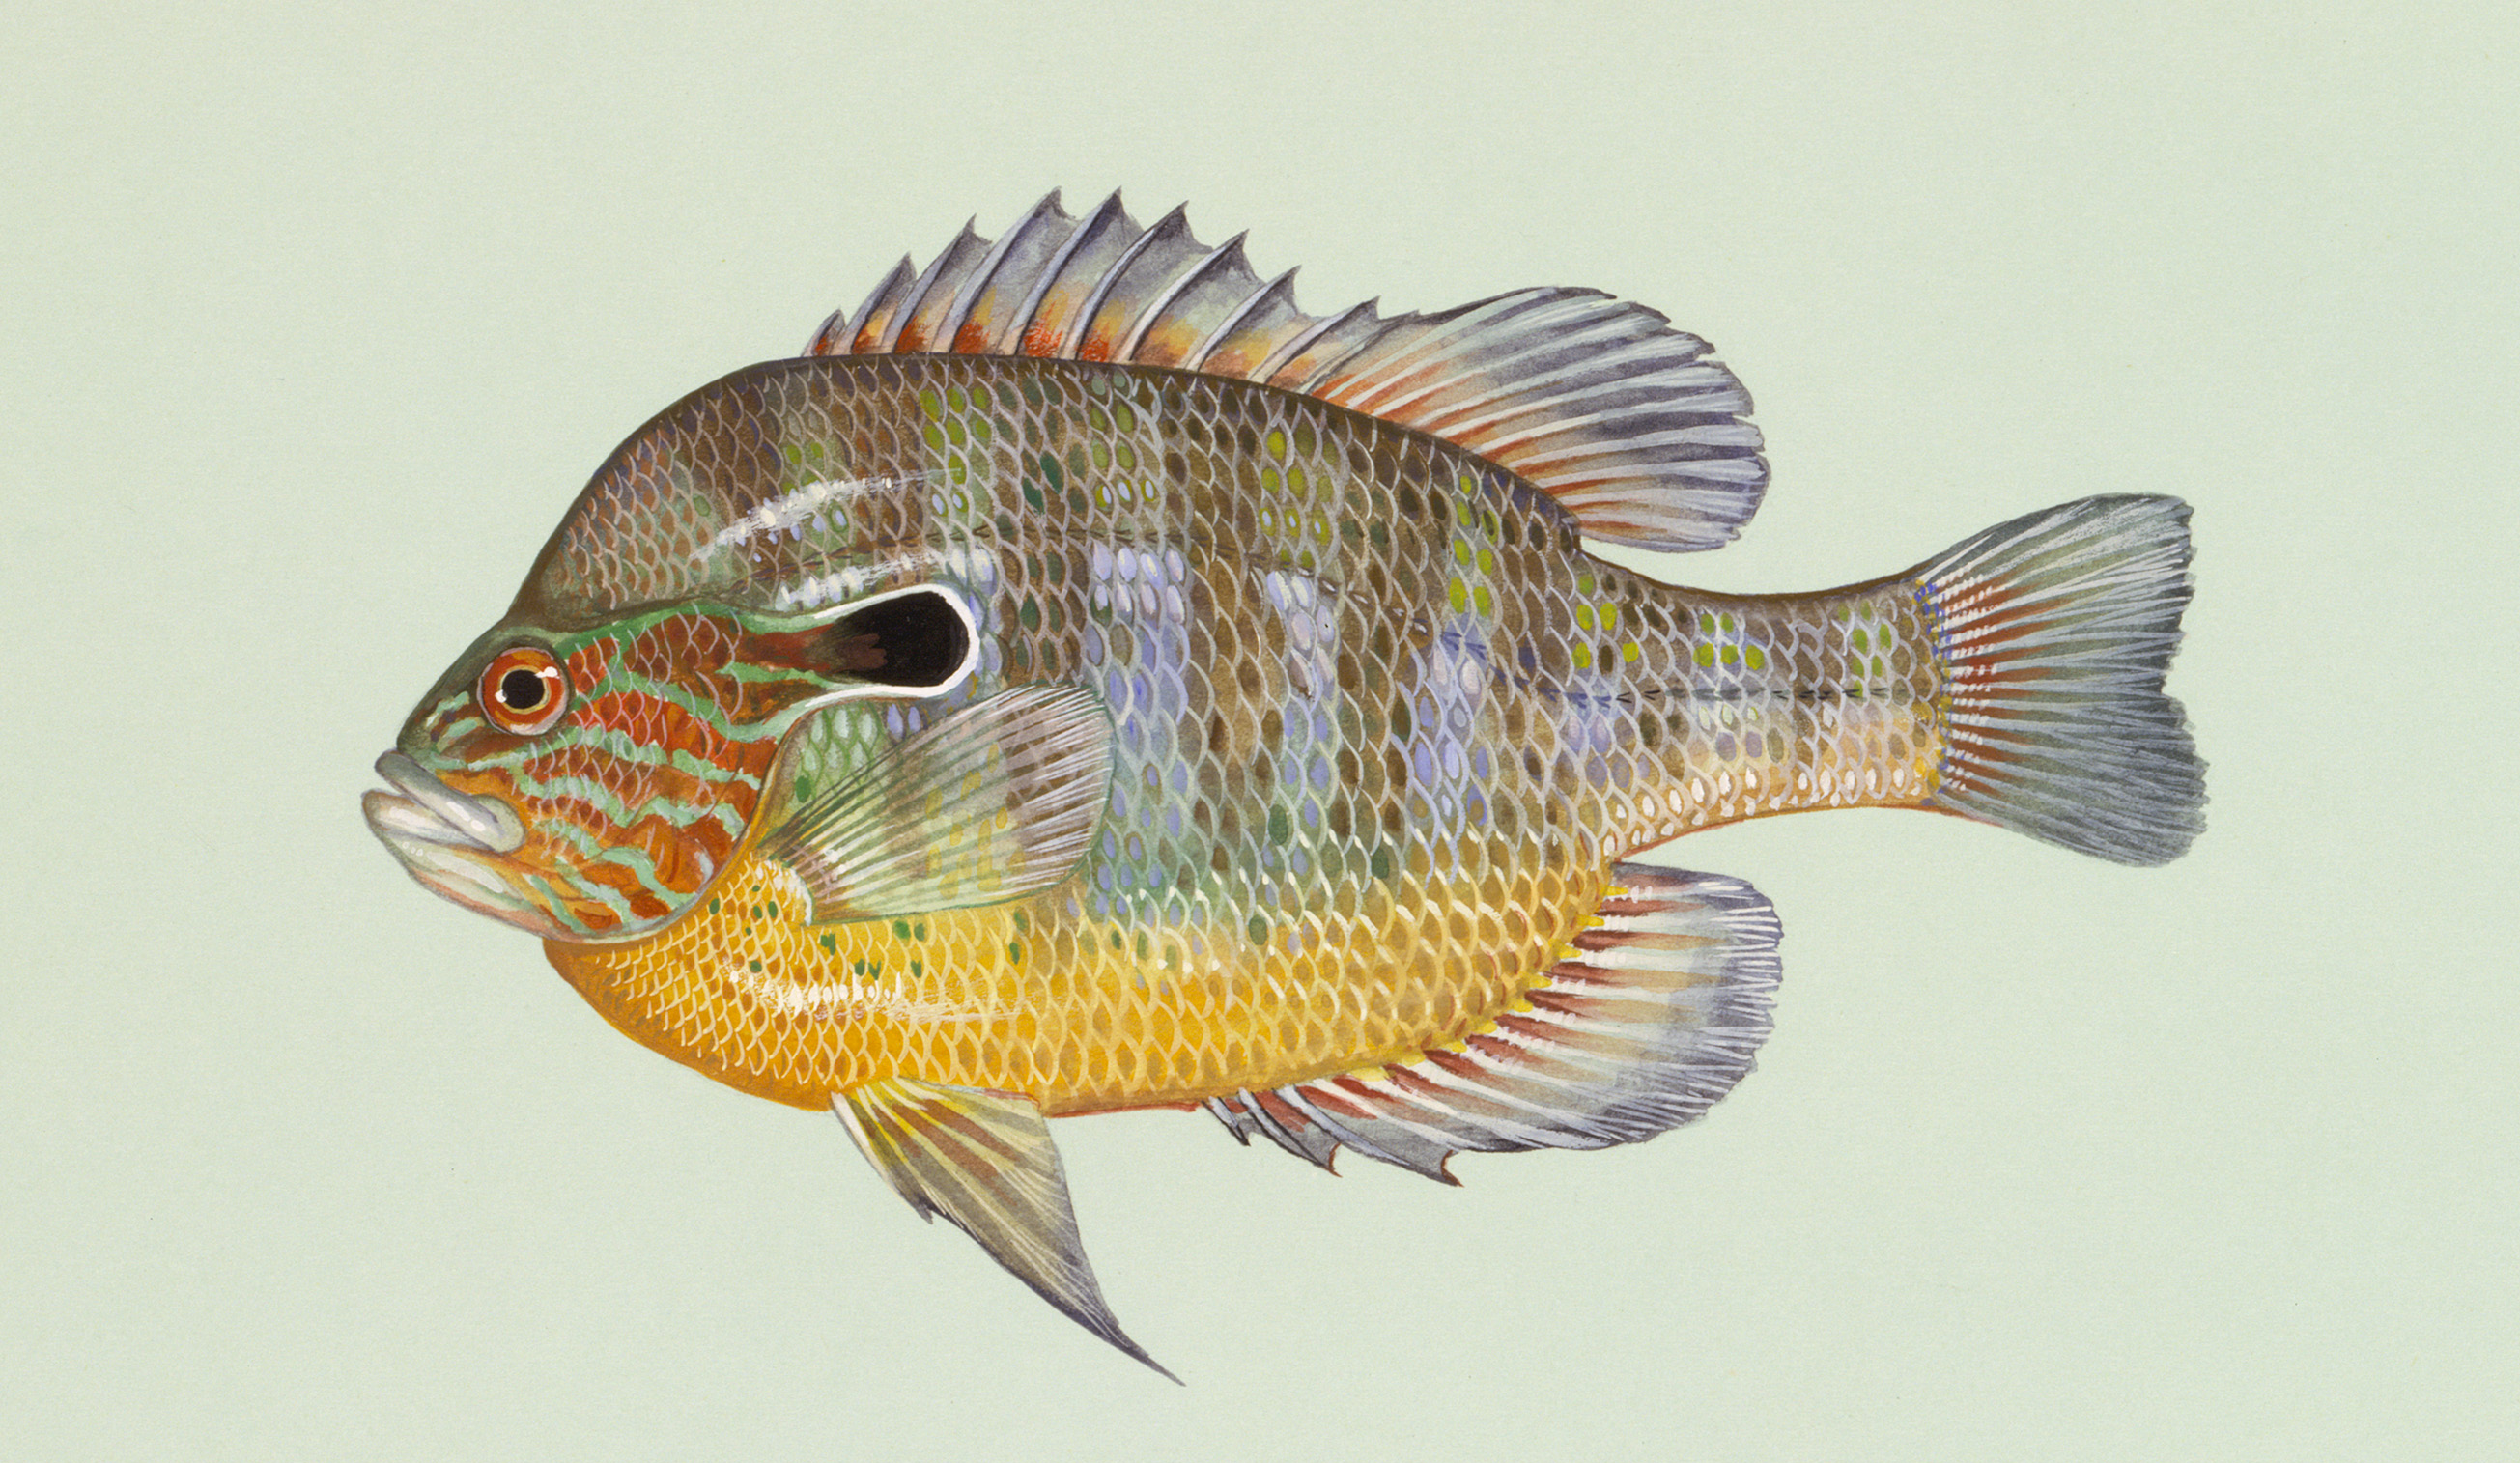
\includegraphics[scale=0.15]{figs/Sunfish/Lepomis_megalotis} %
    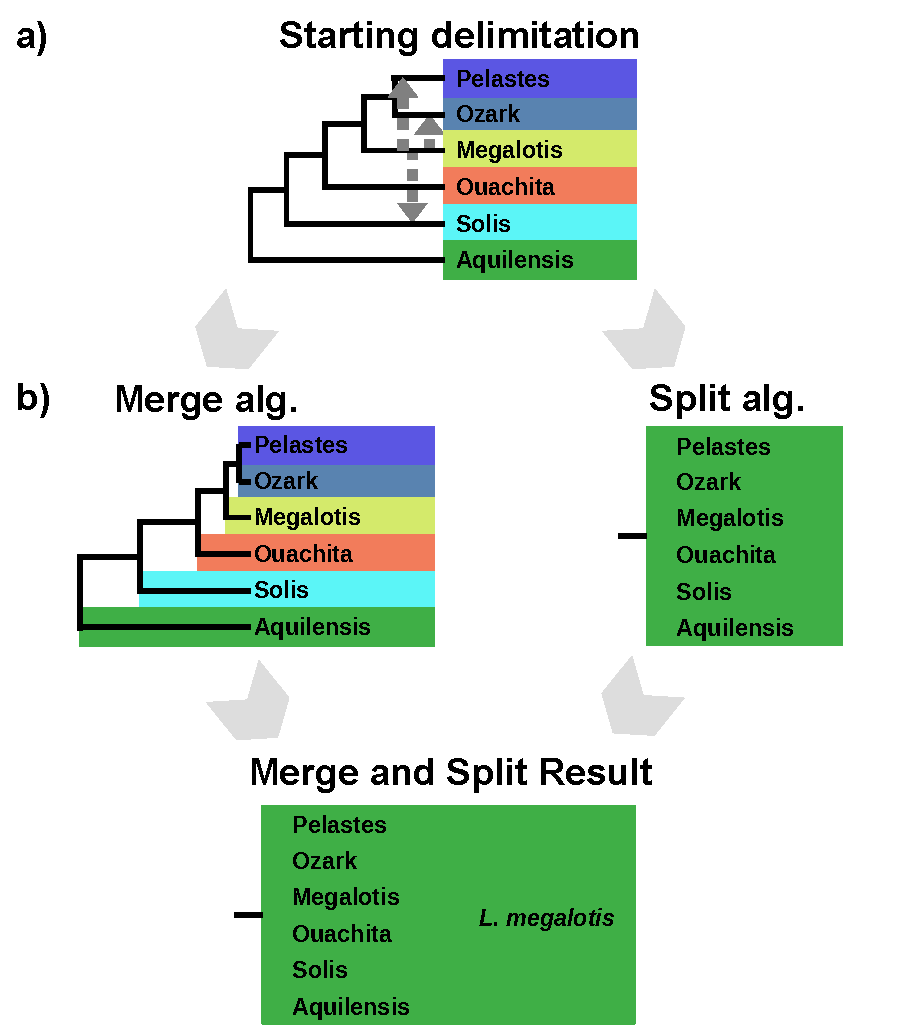
\includegraphics[scale=0.45]{figs/Sunfish/sunfish_results} %
    
    \caption{(\textbf{a}) The guide tree (starting delimitation) for the Longear Sunfish
    (\textit{Lepomis megalotis}), with three migration events (from \textit{megalotis} to
    \textit{pelastes}, \textit{solis}, and \textit{ozark}) assumed in the \textsc{bpp}
    analysis, indicated by dotted lines.  %
    (\textbf{b}) Both merge and split algorithms support a single species.  \red{[show
    merge result, as in figures for the other datasets.  We need care to detail, and
    consistency among datasets.]}\blue{[merge and split results are identical, updated figure subtitles to reflect this]}%
    } \label{fig:sunfish}
\end{figure}

The longear sunfish (\textit{Lepomis megalotis}) is a freshwater fish in the sunfish
family, Centrarchidae, of order Perciformes.  It is native to eastern North America from
the Great Lakes down to northeastern Mexico.  Six subspecies are recognised:
\textit{aquilensis}, \textit{solis}, \textit{ouachita}, \textit{megalotis},
\textit{ozark}, and \textit{pelastes}.  Due to widespread geographic distribution and
frequent hybridization, species delimitation in the longear sunfish poses considerable
challenges.

\citet{Kim2022} analyzed a dataset of 163 ddRAD loci (average sequence length 89 bp)
sampled from 50 individuals from the six subspecies.  After determining a species tree
using \textsc{IQ-tree}, they used \textsc{bpp} A00 without migration to calculate $\tau$
and $\theta$ parameters for each of the subspecies, and used these values to calculate
$gdi$ scores, and delimit species in the group.  They found that none of the
populations have $gdi$ values supporting distinct species status. \citet{Kim2022}
also utilized \textsc{Fastsimcoal2} to identify patterns of gene flow, and find evidence
for multiple instances of significant historical or ongoing genetic exchange.

We reanalyzed the data, taking into account migration between the subspecies.  Based on
the hybridization patterns observed by \cite{Kim2022}, migration from \textit{megalotis}
to \textit{pelastes}, \textit{solis}, and \textit{ozark} was specified.  The migration
rate was assigned the gamma prior G($1,100$) with mean 0.01 migrant individuals per
generation.  Merge and split algorithms were run using $gdi$ thresholds of 0.3 and
0.7 (control files in figs.~\ref{fig:sunfish_mcf_merge} \& \ref{fig:sunfish_mcf_split}).

Both merge and split analyses supported a single species.  This is congruent with the
delimitation of \citet{Kim2022}, who calculated $gdi$ under the MSC model without
gene flow.  \red{[look at parameter estimates.]}


%\newpage

\section{Discussion}

\subsection{Challenges of heuristic species delimitation}

In this paper we have developed a python pipeline to automate the procedure of
hierarchical merge and split algorithms of heuristic species delimitation, initially
discussed by \citet{Leache2019}.  Our tests using both simulated and empirical datasets
suggest that the implementation is correct, and the approach is less likely to suffer
from over-splitting, which has been discussed extensively as a problem with the approach
of Bayesian model selection \citep{Yang2010}.  We expect that the new implementation
will be useful when evolutionary biologists want to integrate evidence based on
multilocus genetic or genomic data in an integrated approach to species delimitation
\citep{Fujita2012}.  The pipeline allows one to utilize the power of the MSC framework
and the \textsc{bpp} program to estimate population parameters precisely and accurately
using the ever-increasing genomic sequence data.

One should not expect the $gdi$ or our pipeline to be a panacea that will apply to all
cases of species delimitation problems using genomic data. First, we note that the $gdi$
criterion and thus our pipeline may suffer from ambiguities.  Suppose there are $K$
populations on the guide tree, the merge algorithm may arrive at a high number of
species ($K_u$) while the split algorithm at a low number ($K_l$), with $1 \le K_l \le
K_u \le K$.  When the two algorithms disagree, the $gdi$ is ambiguous
\citep{Jackson2017}.   Another ambiguity concerns the definition of $gdi$.  In
eqs.~\ref{eq:gdi} or \ref{eq:gdi-mscm}, we considered a sample of two $A$ sequences and
one $B$ sequence.  Similarly one may consider two $B$ sequences and one $A$ sequence.
Under the MSC model of no gene flow, the two definitions are
\begin{equation}
   \begin{aligned}
      gdi_A = 1 - \e^{-2\tau _{AB}/\theta_A} , \\
      gdi_B = 1 - \e^{-2\tau _{AB}/\theta_B}
   \end{aligned}
\end{equation}
(cf: eq.~\ref{eq:gdi}).  When $A$ and $B$ have very different population sizes
($\theta_A, \theta_B$), the two definitions may be inconsistent concerning the species
status of $A$ and $B$.  For example, $A$ may appear to be a different species from $B$
judged by $gdi_A$, but $B$ may not appear to be a distinct species from $A$ judged by
$gdi_B$ \citep{Leache2019}.  One may insist on both $gdi_A$ and $gdi_B$ exceeding the
threshold in our pipeline.

Second, a large $gdi$ may result from a very small population size even if the
divergence time is small.  It may be advisable to examine the population size or the
absolute divergence time together with the $gdi$ \citep{Rannala2020}.

We note that alternative heuristic criteria can be similarly used in our pipeline.  In
particular, composite criteria can be used to determine the species status.  For
example, we may insist, besides the $gdi$ cutoff, that the species split time reach a
minimum of $10^4$ generations \citep{Rannala2020} or the migration rate between the two
species cannot exceed $M = Nm = 0.1$ migrants per generation.

\subsection{Gene flow and species status}

Analyses of genomic data in the past two decades have demonstrated the prevalence of
interspecific gene flow.  Several studies suggested evidence for speciation despite
ongoing gene flow, as in \textit{Heliconius} butterflies \citep{Martin2013}, Mangrove
trees \citep{He2019}, and Western Pacific abalones \citep{Hirase2021}.  Good species are
recognised even if there is significant evidence for gene flow between them.

It is not so clear how to incorporate gene flow in the hierarchical merge and split
algorithms.  In the framework of Bayesian model selection, there are three models or
scenarios for two populations $A,B$: (i) $M_1$ one species, (ii) $M_{20}$ Two species
with no gene flow, and (iii) $M_{21}$ two species with gene flow.  \citet{Leache2019}
compare $M_1$ and $M_{20}$ to decide whether there are one or two species. Alternatively
one may insist on species status only if there is no significant amount of gene flow
(i.e., only if $M_{20}$ wins over both $M_1$ and $M_{21}$).  This approach may suffer
from over-lumping.

In \citet{Leache2019}, we used MSC with no gene flow to construct the guide tree and to
calculate the $gdi$.  The resulting guide tree \citep[][figure 3b]{Leache2019} was
incorrect, even though it led to the correct inference of two species ($ABCD$ and $X$). 
If we use the correct MSC-M model and correct guide tree of figure \ref{fig:ABCDX}a, the
hierarchical merge and split algorithms will never recover the correct delimitation of
two species.  One approach may be to allow the merge of populations that exchange
migrants at a certain rate even if they are not sister lineages on the guide tree.  For
example, in the case of figure \ref{fig:ABCDX}a, we may attempt to merge $AB$, $BC$, and
$CD$, if the migration rate between the species pairs exceed a certain threshold.

\subsection{The guide tree and paraphyletic species}

Our pipeline requires the user to supply a guide tree.  This may be inferred using a
species tree estimation method under the MSC model with no gene flow \citep{Yang2014,
Rannala2017}.  Alternatives include maximum likelihood tree inference using concatenated
data, or use of the mitochondrial genes.

We note that the hierarchical merge and split algorithms do not work when a species is
paraphyletic.  The guide tree of figure \ref{fig:ABCDX} is such an example.  Can we
think of any ideas for delimiting paraphyletic species?  In the case of no gene flow,
paraphyletic species does not seem to make sense.  When there is gene flow between the
geographic populations of the paraphyletic species, perhaps we can allow the merging of
such populations if there is significant evidence for gene flow.  This problem exist for
the reversible-jump algorithms of \citet{Yang2010} as well.

Note that the discussion here concerns the non-monophyly of the populations, rather than
non-monophyly of gene trees, which is known to be problematic if used to delimit species
\cite{Knowles2007}.

Cite \citet{Sukumaran2021, Solis-Lemus2015}.  


\section{Program availability}

The pipeline is written in python, which drives parameter estimation under the MSC or
MSC-M models using \textsc{bpp}.  The source code, documentation, and empirical datasets
analyzed in the paper are available at \texttt{\small https://github.com/abacus-gene/xxx}.

\section{Acknowledgements} 

We thank Bruce Rannala for code for calculating average pairwise sequence distances
between species and Asif Tamuri for help reviewing the code.  This study has been
supported by Biotechnology and Biological Sciences Research Council grants (BB/T003502/1,
BB/R01356X/1) to Z.Y.

%\newpage
\bibliographystyle{natbib}
\renewcommand{\bibfont}{\scriptsize}
\bibliography{bppGDI}


%\begin{landscape}
%%%
%%% SI figures and tables
\newpage
\FloatBarrier %
\setcounter{table}{0} %
\setcounter{figure}{0} %
\renewcommand{\thetable}{S\arabic{table}} %
\renewcommand{\thefigure}{S\arabic{figure}} %

\newpage
*
\newpage

\begin{figure}[h]
	\footnotesize
    \begin{verbatim}
# output
output_directory = res_sim_merge

# input files
Imapfile = Leache_2019_starting_populations.txt
seqfile = Leache_2019_sequences.txt

# guide tree
guide_tree = ((A, B), (C, D)), X);

# hierarchical algo. parameters
mode = merge
GDI threshold = <0.2

# MCMC settings
threads = 4
burnin = 50000
nsample = 100000
\end{verbatim}

\caption{Control file for the ABCDX merge analysis (see
figs.~\ref{fig:ABCDX_out}\&\ref{fig:ABCDX_text_out}).  \texttt{output\_directory}
specifies the directory in which result files will be written.  \texttt{seqfile} is the
sequence alignment file in \textsc{phylip} formatt. \texttt{Imapfile} specifies the
mapping of individuals to populations. \texttt{guide\_tree} is a Newick representation of
the guide tree topology.  \texttt{mode} specifies the algorithm (\texttt{merge} or
\texttt{split}). \texttt{GDI\_threshold} specifies the $gdi$ value below which two
populations are merged into a candidate species.  \texttt{threads} specifies the number of
cpu threads used to run \textsc{bpp}.  \texttt{burnin}, \texttt{nsample} and
\texttt{sampfreq} specify the MCMC settings for run \textsc{bpp}. %
} \label{fig:ABCDX_mcf}
\end{figure}



\begin{figure}
\centering
\footnotesize

\begin{verbatim}
Number of species in starting delimitation:  5
((A, B), (C, D)), X);

*** Iteration 1 ***

Inferred tau and theta parameters:
        theta   tau
X       0.0098	
A       0.0138	
B       0.0202	
C       0.0212	
D       0.0263	
ABCDX   0.0368  0.0101
ABCD    0.0432  0.0006
AB      0.0128  0.0003
CD      0.0204  0.0002

Proposal results:
Node pair        gdi 1   gdi 2   merge accepted?
'A', 'B'         0.05    0.03    True
'C', 'D'         0.03    0.02    True

Number of species after iteration 1:  3
((AB, CD), X);

*** Iteration 2 ***

Inferred tau and theta parameters:
        theta   tau
X       0.0098	
AB      0.0194	
CD      0.0286	
ABCDX   0.0367  0.0101
ABCD    0.0428  0.0006

Proposal results:
Node pair        gdi 1   gdi 2   merge accepted?
'AB', 'CD'       0.07    0.05    True 

Number of species after iteration 2:  2
(ABCD, X);

*** Iteration 3 ***

Inferred tau and theta parameters:
        theta   tau
X       0.0098
ABCD    0.0441	
ABCDX   0.0365  0.0102


Proposal results:
Node pair        gdi 1   gdi 2   merge accepted?
'ABCD', 'X'      0.39    0.87    False

Number of species after iteration 3:  2
(ABCD, X);

Final delimitation reached.
\end{verbatim}
 
\caption{Screen output from running the hierarchical merge algorithm to analyze the
simulated dataset of figure \ref{fig:ABCDX}. %
} \label{fig:ABCDX_text_out}
\end{figure}

\begin{figure}[h]
\footnotesize
\begin{verbatim}

# Notes: species are renamed as follows
#
# gir_ang = giraffa+angolensis
# tip_tho = tippelskirchi+thornicrofti
# cam_rot_ant = camelopardalis+rothschildi+antiquorum
# per = peralta
# ret = reticulata
		
# output
output_directory = res_giraffe_merge

# input files
Imapfile = Imap_Giraffe.txt
seqfile = MSA_Giraffe.txt

# guide tree
guide_tree = ((gir_ang,tip_tho),((cam_rot_ant,per),ret));

# migration events and priors
migration = {
    ret -> tip_tho,
    tip_tho -> ret,
    ret -> cam_rot_ant,
    cam_rot_ant -> ret,
}
migprior = 0.1 10

# hierarchical algorithm settings
mode = merge
gdi_threshold = <0.3

# MCMC settings
threads = 4
burnin = 50000
nsample = 200000
sampfreq = 2
\end{verbatim}

\caption{Control file for the merge algorithm in analysis of the Giraffes data. The
results are in figure \ref{fig:giraffe}. %
} \label{fig:giraffe_mcf_merge}
\end{figure}

\begin{figure}[h]
\footnotesize
\begin{verbatim}
# output
output_directory = res_giraffe_split

# input files
Imapfile = Imap_Giraffe.txt
seqfile = MSA_Giraffe.txt

# guide tree
guide_tree = ((gir_ang,tip_tho),((cam_rot_ant,per),ret));

# migration events and priors
migration = {
 ret -> tip_tho,
 tip_tho -> ret,
 ret -> cam_rot_ant,
 cam_rot_ant -> ret,
}
migprior = 0.1 10

# hierarchical algo. parameters
mode = split
gdi_threshold = >0.7

# MCMC settings
threads = 4
burnin = 50000
nsample = 200000
sampfreq = 2
\end{verbatim}

\caption{Control file for the split analysis in Giraffes data.  The results are in
figure \ref{fig:giraffe}. %
} \label{fig:giraffe_mcf_split}
\end{figure}




\begin{figure}[h]
\footnotesize
\begin{verbatim}
# Notes: species are renamed as follows
#
# Po = polyzona
# Ab = abnorma
# Mi = micropholis
# An = annulata
# Ge = gentilis
# Tr = triangulum
# El = elapsoides

# output
output_directory = res_milksnake_merge

# input files
Imapfile = Imap_Lampropeltis.txt
seqfile = MSA_Lampropeltis.txt

# guide tree
guide_tree = (((Po, (Ab, Mi)), (An, (Ge, Tr))), El);

# hierarchical algorithm settings
mode = merge
gdi_threshold = <0.3

# MCMC settings
threads = 4
burnin = 50000
nsample = 200000
sampfreq = 2
\end{verbatim}

\caption{Control file for the merge analysis of the Milksnakes data.  The results are 
presented in figure \ref{fig:milksnake}. %
} \label{fig:milksnake_mcf_merge}
\end{figure}

\begin{figure}[h]
\footnotesize
\begin{verbatim}
# output
output_directory = output_directory = res_milksnake_split

# input files
Imapfile = Imap_Lampropeltis.txt
seqfile = MSA_Lampropeltis.txt

# guide tree
guide_tree = (((Po, (Ab, Mi)), (An, (Ge, Tr))), El);

# hierarchical algorithm settings
mode = split
gdi_threshold = >0.7

# MCMC settings
threads = 4
burnin = 50000
nsample = 200000
sampfreq = 2
\end{verbatim}

\caption{Control file for the split analysis of the Milksnakes data.  The results are
presented in figure \ref{fig:milksnake}. %
} \label{fig:milksnake_mcf_split}
\end{figure}

\begin{figure}[h]
\footnotesize
\begin{verbatim}
# output
output_directory = # will be set from the command line

# input files
Imapfile = # will be set from the command line
seqfile = trigentalt.txt

guide_tree = ((Ge,Tr),Al);

mode = merge
gdi_threshold = <0.3

threads = 4
burnin = 50000
nsample = 100000
sampfreq = 2
\end{verbatim}

\caption{Control file for the analysis of the milksnake data under delimitation
hypotheses reflecting the East-West splits.  The results are presented in figure
\ref{fig:milksnake}.  The \texttt{Imapfile} and \texttt{output\_directory} parameters are
left empty, as they will be provided at the command line, to ensure that the same basic
control file can be used for each of the five alternative East-West delimitations. %
} \label{fig:milksnake_EW_mcf}
\end{figure}

\begin{figure}[h]
\footnotesize
\begin{verbatim}
HMDelimit --mcfile mcf_milksnake_EW.txt --mcfpor \
Imapfile = trigent1alt.Imap.txt, output_directory = res_EW_1 

HMDelimit --mcfile mcf_milksnake_EW.txt --mcfpor \
Imapfile = trigent2alt.Imap.txt, output_directory = res_EW_2 

HMDelimit --mcfile mcf_milksnake_EW.txt --mcfpor \
Imapfile = trigent3alt.Imap.txt, output_directory = res_EW_3 

HMDelimit --mcfile mcf_milksnake_EW.txt --mcfpor \
Imapfile = trigent4alt.Imap.txt, output_directory = res_EW_4 

HMDelimit --mcfile mcf_milksnake_EW.txt --mcfpor \
Imapfile = trigent5alt.Imap.txt, output_directory = res_EW_5
\end{verbatim}

\caption{Shell script used to iterate through alternative East-West delimitation
hypotheses in Milksnakes, presented in figure \ref{fig:milksnake}. The \texttt{-mcfpor}
(control file parameter override) flag is used to override parameters of the mcf via the
command line interface, setting the Imap file to one of the alternative East-West
delimitations, and specifying the individual output directories for each analysis. %
} \label{fig:milksnake_EW_shell}
\end{figure}

\begin{figure}[h]
	\footnotesize
	\begin{verbatim}
# Notes: species are renamed:
#
# PEL = pelastes
# OZK = ozark
# MEG = megalotis
# LIT = ouachita
# SOL = solis
# AQU = aquilensis

# output
output_directory = res_sunfish_merge

# input files
Imapfile =  Imap_Sunfish.txt
seqfile = MSA_Sunfish.txt

# guide tree
guide_tree = (((((PEL,OZK),MEG),LIT),SOL),AQU);

# migration events and priors
migration = {
    MEG -> PEL,
    MEG -> SOL,
    MEG -> OZK
}
migprior = 0.1 10

# hierarchical algo. parameters
mode = merge
gdi_threshold = <0.3

# MCMC settings
threads = 4
burnin = 50000
nsample = 200000
sampfreq = 2
\end{verbatim}

\caption{Control file for the merge analysis of the sunfish data.  The results are
presented in figure \ref{fig:sunfish}. %
} \label{fig:sunfish_mcf_merge}
\end{figure}

\begin{figure}[h]
\footnotesize
\begin{verbatim}
# output
output_directory = res_sunfish_split

# input files
Imapfile =  Imap_Sunfish.txt
seqfile = MSA_Sunfish.txt

# guide tree
guide_tree = (((((PEL,OZK),MEG),LIT),SOL),AQU);

# migration events and priors
migration = {
    MEG -> PEL,
    MEG -> SOL,
    MEG -> OZK
}
migprior = 0.1 10

# hierarchical algo. parameters
mode = split
gdi_threshold = >0.7

# MCMC settings
threads = 4
burnin = 50000
nsample = 200000
sampfreq = 2
\end{verbatim}

\caption{Control file for the split analysis of the sunfish data.  The results are
presented in figure \ref{fig:sunfish}. %
} \label{fig:sunfish_mcf_split}
\end{figure}


\onecolumn

\begin{sidewaystable}
	\vspace{5.5in}
	\begin{small}
		\caption{Rate matrix for Markov chain describing transitions between states in
			multispecies coalescent with migration model with two populations ($A$ and $B$) and three
			sequences ($a_1$, $a_2$, and $b$). %
		} \label{table:Q}
		\begin{tabular}{lccccccccccccccccccccccc} 
			\toprule
			& $AAA$ & $AAB$ & $ABA$ & $ABB$ & $BAA$ & $BAB$ & $BBA$ & $BBB$ & $A_{a_1}A$ & $A_{a_2}A$ & $A_{b}A$ & $C_{a_1}B$ & $B_{a_2}B$ & $B_{b}B$ & $A_{a_1}B$ & $A_{a_2}B$ & $A_{b}B$ & $AB_{a_1}$ & $AB_{a_2}$ & $AB_{b}$ & $A|B$ \\  
			\midrule
			$AAA$ & $\cdot$ & $w_{BA}$ & $w_{BA}$ & & $w_{BA}$ & & & & $c_A$ & $c_A$ & $c_A$ & & & & & & & & & & \\ 
			$AAB$ & $w_{AB}$ & $\cdot$ & & $w_{BA}$ & & $w_{BA}$ & & & & & & & & & & & & & & $c_A$ & \\
			$ABA$ & $w_{AB}$ & & $\cdot$ & $w_{BA}$ & & & $w_{BA}$ & & & & & & & & & & & & $c_A$ & & \\
			$ABB$ & & $w_{AB}$ & $w_{AB}$ & $\cdot$ & & & & $w_{BA}$ & & & & & & & $c_B$ & & & & & & \\
			$BAA$ & $w_{AB}$ & & & & $\cdot$ & $w_{BA}$ & $w_{BA}$ & & & & & & & & & & & $c_A$ & & & \\
			$BAB$ & & $w_{AB}$ & & & $w_{AB}$ & $\cdot$ & & $w_{BA}$ & & & & & & & & $c_B$ & & & & & \\
			$BBA$ & & & $w_{AB}$ & & $w_{AB}$ & & $\cdot$ & $w_{BA}$ & & & & & & & & & $c_B$ & & & & \\
			$BBB$ & & & & $w_{AB}$ & & $w_{AB}$ & $w_{AB}$ & $\cdot$ & & & & $c_B$ & $c_B$ & $c_B$ & & & & & & & \\
			$A_{a_1}A$ & & & & & & & & & $\cdot$ & & & & & & $w_{BA}$ & & & $w_{BA}$ & & & $c_A$ \\
			$A_{a_2}A$ & & & & & & & & & & $\cdot$ & & & & & & $w_{BA}$ & & & $w_{BA}$ & & $c_A$ \\
			$A_bA$ & & & & & & & & & & & $\cdot$ & & & & & & $w_{BA}$ & & & $w_{BA}$ & $c_A$ \\
			$B_{a_1}B$ & & & & & & & & & & & & $\cdot$ & & & $w_{AB}$ & & & $w_{AB}$ & & & $c_B$ \\
			$B_{a_2}B$ & & & & & & & & & & & & & $\cdot$ & & & $w_{AB}$ & & & $w_{AB}$ & & $c_B$ \\
			$B_bB$ & & & & & & & & & & & & & & $\cdot$ & & & $w_{AB}$ & & & $w_{AB}$ & $c_B$ \\
			$A_{a_1}B$ & & & & & & & & & $w_{AB}$ & & & $w_{BA}$ & & & $\cdot$ & & & & & & \\
			$A_{a_2}B$ & & & & & & & & & & $w_{AB}$ & & & $w_{BA}$ & & & $\cdot$ & & & & & \\
			$A_bB$ & & & & & & & & & & & $w_{AB}$ & & & $w_{BA}$ & & & $\cdot$ & & & & \\
			$AB_{a_1}$ & & & & & & & & & $w_{AB}$ & & & $w_{BA}$ & & & & & & $\cdot$ & & & \\
			$AB_{a_2}$ & & & & & & & & & & $w_{AB}$ & & & $w_{BA}$ & & & & & & $\cdot$ & & \\
			$AB_b$ & & & & & & & & & & & $w_{AB}$ & & & $w_{BA}$ & & & & & & $\cdot$ & \\
			$A|B$ & & & & & & & & & & & & & & & & & & & & & $\cdot$ \\
			\bottomrule
		\end{tabular}
		
		\noindent Note.--- $w_{AB} = 4M_{AB}/\theta_B = m_{AB}/\mu$ and $w_{BA} =
		4M_{BA}/\theta_A = m_{BA}/\mu$ are mutation-scaled migration rates, and $c_A =
		2/\theta_A$ and $c_B = 2/\theta_B$ are the coalescent rates, when one time unit is the
		expected time to accumulate one mutation per site.  The state of the chain is given by
		the population IDs ($A$ or $B$) and sequence IDs. For example the initial state
		$A_{a_1}A_{a_2}B_b$ means that the three sequences $a_1, a_2$, and $b$ are from
		populations $A$, $A$, and $B$, respectively.  States with three sequences are
		abbreviated, with the three sequences assumed to be in the order $a_1, a_2, b$ so that
		the sequence IDs are suppressed.  Thus $A_{a_1}A_{a_2}B_b$ is `$AAB$'.  State
		$A_{a_1a_2}B_b$ means that two sequences remain in the sample, with the ancestor of
		sequences $a_1$ and $a_2$ is in population $A$ while sequence $b$ is in population
		$B$. This is abbreviated `$AB_b$', with the sequence ID `$a_1a_2$' suppressed. `$A|B$'
		is an absorbing state in which only one sequence remains in the sample, in either $A$
		or $B$, after two coalescent events have occurred.  From \citet{Leache2019}.
	\end{small}
\end{sidewaystable}

\end{document}
